\documentclass[a4paper, 11pt]{report}
\usepackage{cite}
\usepackage{blindtext}
\usepackage[T1]{fontenc}
\usepackage[utf8]{inputenc}
\usepackage{titlesec}
\usepackage{fancyhdr}
\usepackage{geometry}
\usepackage{fix-cm}
\usepackage[hidelinks]{hyperref}
\usepackage{graphicx}
\usepackage{multirow}
\usepackage[english]{babel}
\geometry{ margin=30mm }
\counterwithin{subsection}{section}
\renewcommand\thesection{\arabic{section}.}
\renewcommand\thesubsection{\thesection\arabic{subsection}.}
\usepackage{tocloft}
\renewcommand{\cftchapleader}{\cftdotfill{\cftdotsep}}
\renewcommand{\cftsecleader}{\cftdotfill{\cftdotsep}}
\setlength{\cftsecindent}{2.2em}
\setlength{\cftsubsecindent}{4.2em}
\setlength{\cftsecnumwidth}{2em}
\setlength{\cftsubsecnumwidth}{2.5em}


\begin{document}
\titleformat{\section}
{\normalfont\fontsize{15}{0}\bfseries}{\thesection}{1em}{}
\titlespacing{\section}{0cm}{0.5cm}{0.15cm}
\titleformat{\subsection}
{\normalfont\fontsize{13}{0}\bfseries}{\thesubsection}{0.5em}{}
\titlespacing{\section}{0cm}{0.5cm}{0.15cm}

%=======================================================================================

% #########################
% IMPORTANT - Add student names here!
% e.g. \newcommand{\stud1}{LOWE, David}
\newcommand{\studA}{{Hilton, Naidu}}
\newcommand{\studB}{{Li, Yunheng}}
\newcommand{\studC}{{Donaldson, Jake}}
\newcommand{\studD}{{Zhang, Andrew}}
% ADD ANOTHER LINE FOR A FIFTH MEMBER
%
% IMPORTANT - Then give your SIDs
\newcommand{\sidA}{{550770402}}
\newcommand{\sidB}{{540101492}}
\newcommand{\sidC}{{550748788}}
\newcommand{\sidD}{{540750773}}
% ADD ANOTHER LINE FOR A FIFTH MEMBER

%
% IMPORTANT - And then update which major each student will focus on
\newcommand{\majA}{{Computer Science}}
\newcommand{\majB}{{Data Science}}
\newcommand{\majC}{{SW Development}}
\newcommand{\majD}{{Cyber Security}}
% ADD ANOTHER LINE FOR A FIFTH MEMBER - HCI

% #########################


\pagenumbering{Alph}
\begin{titlepage}
\begin{flushright}

\includegraphics[width=4cm]{USyd.jpg}\\[1cm]
\end{flushright}

\begin{centering}
\textbf{\huge INFO1111: Computing 1A Professionalism}\\[0.75cm]
\textbf{\huge 2025 Semester 1}\\[2cm]
\textbf{\huge Skills: Team Project Report}\\[2cm]

\textbf{\large Submission number: 1}\\[0.5cm]
\textbf{\large Github link: https://github.com/Hilton-Naidu/SkillsProject1.git }\\[0.75cm]
\textbf{\huge Team Members: 4}\\[0.75cm]

\begin{tabular}{|p{0.25\textwidth}|p{0.13\textwidth}|p{0.12\textwidth}|p{0.12\textwidth}|p{0.22\textwidth}|}
	\hline
	\multirow{2}{*}{Name} & \multirow{2}{*}{Student ID} & Target * & Target * & \multirow{2}{*}{Selected Major} \\
	 & & Foundation & Advanced & \\
	\hline
	\hline
	\raggedright{\studA} & \sidA & S & A & \majA \\
	\hline
	\raggedright{\studB} & \sidB & S & A & \majB \\
	\hline
	\raggedright{\studC} & \sidC & A & NA & \majC \\
	\hline
	\raggedright{\studD} & \sidD & A & NA & \majD \\
	\hline
\end{tabular}
\\[0.5cm]
\end{centering}

* Use the following codes:
\begin{itemize}
\setlength\itemsep{0em}
\item NA = Not attempting in this submission
\item A = Attempting (not previously attempting)
\item AW = Attempting (achieved weak in a previous submission) 
\item AG = Attempting (achieved good in a previous submission)
\item S = Already achieved strong in a previous submission
\end{itemize}

\thispagestyle{empty}
\end{titlepage}
\pagenumbering{arabic}


%=======================================================================================

\tableofcontents

%=======================================================================================



%=======================================================================================

\newpage
\section{Task 1 (Foundation): Core Skills}
Hello
Throughout your Computing degree we will help you learn a range of new skills. Once you graduate however you will need to continue to learn new languages, new tools, new applications, etc. Task 1 focuses on core technical skills (related to \LaTeX\ and Git) and the key technical skills used in different computing jobs. Each member of the team should individually complete their subsection below. You should begin by allocating to each team member a different major to focus on (i.e. one of: Computer Science; Data Science; Software Development; Cyber Security). If you have a fifth member, then your tutor will suggest a fifth topic to cover. This allocation should be specified above (see lines 37-56 in the LaTeX file).

Each member of your team is required to select one of the designated domains and collaboratively work on the scenario presented below. The primary objective is to reflect on the collaborative process and problem-solving strategies rather than solely focusing on the final solution.

The focus is on your team’s collaborative process and problem solving skills rather than the solution itself. 

You will need to integrate your information into this shared collaborative LaTeX document and compile the result.\\[2mm]

Foundation is based on 3 components:\\[1mm]

\textbf{Scenario: Collaborative Disaster Response System Development}

{\begin{quote}\itshape
With devastating natural disasters, such as the 2025 LA wildfires, communication between emergency services, volunteers, and affected communities is chaotic and inefficient.

Develop an approach to streamline communication and optimise resource distribution during such crises. 
\end{quote}}

\textbf{ROLES:}
\begin{itemize}
    \item Computer Science (CS) domain develops the system infrastructure and applications to allow for integration between emergency services, databases, volunteers, and affected people. They will need to ensure this is automated and efficient in allocating resources.
    \item Software Engineering (SE) will ensure the infrastructure is scalable and robust to manage unpredictability of material disasters and amount of people affected. The system must have offline capabilities since natural disasters can disrupt telecommunications. They will make sure the infrastructure runs smoothly and ensures its user friendly.
    \item Cybersecurity protects communication channels from disruptions or hacks, protects personal data and ensures that access to confidential information is managed appropriately by authorised personnel. They will need to implement measures to mitigate false reporting or misinformation.
    \item Data Science (DS) will use analytics including data visualisation to forecast natural disasters from historical and real time data. They need to identify high risk areas from multiple sources of data to optimise resource allocation, routes and most urgent areas of need for emergency responders.
    \item If there is a 5th group member, Human-Computer Interaction (HCI) will ensure the system is intuitive and accessible for all users. This includes usability testing and refining the application and focusing on User Experience and Interaction (UI and UX) design.
\end{itemize}

\textbf{Component 1 Project management / technical skills:}

The team is required to create a project on GitHub and manage their tasks using GitHub’s issue tracking system.

\begin{itemize}
    \item Create a project within your GitHub repository
    \item Define tasks as issues and assign them to team members
    \item Track task progress throughout the project lifecycle
    \item Mark issues as resolved upon completion
\end{itemize}
For example, issue: ‘research 2 technical skills for Data Science’ and assign to John Applesmith. \\[2mm]

\textbf{Component 2 Group questions:}

\begin{itemize}
    \item Describe your team’s collaborative process in developing a solution.
    \item How did you approach the problem as a team, and what challenges did you encounter in working together? 
    \item Discuss how your team arrived at your final approach, including the decision-making process, compromises made, and key turning points. 
\end{itemize}
Target: 300-500 words \\[2mm]

\textbf{Component 3 Individual questions:}
\begin{itemize}
    \item Reflect on the skills relevant to your domain that were essential for this project. What technical or professional skills have you identified were relevant to the project? Refer to the Skills Framework for the Information Age (SFIA) list of skills \cite{sfia} and describe at least 2 skills per domain. 
    \item How did working collaboratively on this project help you strengthen those skills? 
    \item What professional or technical skills have you identified you need to develop or fine-tune?
\end{itemize}

Target: 300-400 words \\[2mm]


\textbf{OVERALL REQUIREMENTS:}

To achieve an "OK" rating for this task you must individually accomplish the following:
\begin{itemize}
\item Each member of your team \textbf{has been} allocated a different major (Computer Science, Data Science, Software Development, Cyber Security (and Human-Computer Interaction for a fifth member).
\item Submission Contribution section is completed with each subsequent submission
\item Each member of your team \textbf{has identified} 2 key technical skills that you would need to be able to work in the industry of your allocated major.
	\begin{itemize}
	\item Each skill must have an explanation on why it is a key skill required for the industry of the major ($\sim$100 words per skill).
	\item The 2 key tech skills must be identified from the skills framework for the information age SFIA.
	\end{itemize}
\item Github \& LaTeX
	\begin{itemize}
	\item Your team has created a team repository on Github for the project and put a copy of the LaTeX template, bib file, and image file into the team repository (only needs to be done by one member of your team).
    \item \item You have added your tutor to your git repository
    \item Your team has created a GitHub project, created issues and allocated to each member, and closed issues upon completion
	\item The information has been compiled into the shared collaborative LaTeX document using the template provided on Canvas with your team members sections - you have edited the LaTeX template to include your chosen major and responses to both the group discussion questions and individual questions.
	\item You have cloned the team repository to your local machine.
	\item Provide evidence that you can compile from the command line (provide screenshots of the command entered and output).
	\item Provide evidence that you can commit to your local repo (provide screenshots of the steps taken to commit to their local repo).
	\end{itemize}
\item Referencing
	\begin{itemize}
	\item You have provided in-text references (IEEE) to support your claims or where they gathered the information from.
	\item You have a reference list following the IEEE referencing guidelines.
	\item Some common things to look for to see whether your have correctly followed the referencing guide are:
		\begin{itemize}
		\item The sources you have listed are only the sources that are present in-text.
		\item All sources seen in-text are included in the reference list.
		\item You followed the correct convention for references that don’t have author’s details or multiple sources have the same author and year of publication
		\item You have included the required information for the source type as outlined in the guide.
		\item Sources are not a list (i.e. dotpoints)
		\end{itemize}
	\end{itemize}
\end{itemize}

To achieve a "STRONG" rating, you must individually accomplish all of the above in addition to the following:\\
Demonstrate the following to your tutor during the tutorial:
\begin{itemize}
\item You are able to retrieve your team’s shared repo
\item You are able to make changes, recompile, commit changes, and push back to repo.
\item Note: you should also provide screen-shots of relevant actions taken to make changes, recompile etc. does not require you to provide evidence of detailing conflicts.
\end{itemize}


% =======================================================
\subsection{Group response}

For the creation of the solution, we decided to root our collaboration in clearly allocated jobs, allowing us to each act independently while having our work contribute to the progress of others. We concluded that to complete this project, we would need a combination of physical and digital interactions to effectively communicate and stay up to date on the progress.

\subsubsection{Digital:}

For digital communication, we decided to use a social media platform to communicate. We created an online group chat to allow us all to communicate quickly and easily. This medium also had the capability to facilitate group video calls, allowing us to conduct quick meetings when needed. If we were to take this project to full development, we would transition to a more professional medium of communication, such as Microsoft Teams, to allow for the same quick communication but in a platform designed for work.

We also shared collaborative work through the online source repository system, GitHub. Through the use of GitHub, we were able to allocate tasks for each other using the issues functionality, and we were also able to work on a single file together.

The main challenge we encountered in the development of this project was the speed of communication. While we had the capability for almost instantaneous communication, we all had individual lives and, thankfully, were not on our phones constantly. However, this did lead to slower and less effective communication.

\subsubsection{Physical:}

While we did meet once a week at our INFO1111 workshop to work on the project, this was not enough time to complete our group project. Because of this, we decided to have an in-person meeting on the 26th of March from 12:00 till 2:00 in a booked library meeting room. This was a key point in the development of our project and led to the unification of our roles into a single clear development plan.

This also allowed us to use an important medium for idea generation—whiteboards. By doing so, we were able to collaboratively create mind maps and flowcharts for development. If we were fully developing this solution for deployment, we would continue these meetings weekly as a full team while also having smaller pair meetings for different areas to work together on specific aspects, such as DS and CS discussing the efficiency of data communication and compilation.

The two main challenges we encountered with physical communication were absenteeism and personal life schedules. Throughout the period of this project, some people were away at various workshops. While not detrimental, this did significantly limit our ability to collaborate. The second challenge was that, because we are in university and not a work environment, we all have different schedules (work and class) to abide by. This made it difficult to organise in-person meetings, but we overcame this through compromise and early planning.

The following was our approach to breaking down the project and generating a plan for development (creative process):
\begin{itemize}
\item Identify all the parties involved (LAPD, LAFD, Medical Services, Volunteers, Public).
\item The data scientist identified the parameters that would be provided and the types of data that would need to be communicated. We concluded that data from LAPD, LAFD, and Medical Services needed to be combined and unified, with the option to share it with Volunteers and/or the Public.
\item The computer scientist then identified how the system infrastructure would need to be developed to unify the major systems in case of an emergency. He considered the operating system, programming languages, and the integration of backend and frontend logic.
\item From this logic, the software developer identified that due to the unique nature of fire, many electrical (television) and physical methods of communication might be affected. Therefore, he identified how to build robust systems.
\item From these three roles, we created data pathways as follows: (LAPD + LAFD + Medical) → Volunteers → Public.
\item The cybersecurity specialist then identified the areas of data communication and how they might protect the data from a potential attack. While there is always a risk of attack on any digital platform, this project was identified as needing particular focus on cybersecurity due to the sensitive nature of the data being communicated within these systems (medical records, deaths, potential mass fear).
\item After identifying these systems, we then allocated the jobs according to roles, and each person went off to work individually on their area.
\end{itemize}

\subsection{Skills for \majA: \studA}

The relevent skills for a computer scientist to "develops the system infrastructure and applications to allow for integration between emergency services, databases, volunteers, and affected people" according to SFIA 9 Skills are:

\begin{enumerate}
    \item Infrastructure operations (ITOP): Addressing the intergration and operations between various Infrastructures to assure cohesive optimisation accross the project \cite{palma2023}. In this project, ITOP plays an important role in the linkage of virtual, physical and cloud-based environments. Using a strong technical understanding, I  would be able to link the emergency services system, to databases of users, locations, and resources to ensure a optimised communication. 
    \item Solution Architecture (ARCH): Devloping the communication between systems for a multifacuted and multi dimentional solution \cite{palma2023}. For this project this would entail creating a colution whihc takes all existing components, e.g. the emergency systems communication systems made capable for expantion to volunteers. This role ultimatly generates a design for the solution, using technical skiils. .
\end{enumerate}

Working collaboratively significantly helped me by allowing me to interact with my teammates, asking them how their roles behave and how they may contrast or compare with my own to help me get a greater understanding of what to do. For example, when considering one of my Infrastructure operations (ITOP) skill I asked the SW development team make about how my work on intrastructure might be different to his, ensuring we had a significant variation in skills and actions. It also helped to ask what areas had already been covered, to greater ideintify what I needed to do, such as for my Solution Architecture (ARCH) skill, haveing heard all their roles, I was able to identify that a skill area lacking was a indervidual to create an overarching structure and plan for how to act. Ultimatly this allowed me to have a greater undertsanding of my own role, while also  supporting my teammates in their own. 

I have identified that I need to fine tune my Communication skills, and orginisational skills. While I have completed this project, and helped my group with the group aspect, I could have been more foward and active with the orginisational aspect of this project, leading the group meetings and encouraging more only checkups with each other. I could also improve my knowledge, growing my understanding of the more difficult aspects of LaTex and the specific details of how to create different designs. 

The following is a brief summary of my jobs as part of the development of this project:
\begin{itemize}
    \item Identify the operating system (or systems) to be used. Given this Project requires the unification of multiple systems, I need to consider whether creating a custom OS or using an existing one would be the most logical option. This would require consulting the rest of my group. 
    \item I need to deal with creating the capability for the integration of various databases, while it is not my role to deal directly with the data, I should develop some of the mechanics and algorithms to read and write data. 
    \item I need to focus on writing algorithms to automate the communication of data between the LAPD, LAFD, and Medical services. This would require working the DS to determine the type of data being used, and from the trends identified create an automated allocation system to efficiently use resources available. 
\end{itemize}

\begin{figure}[htbp]
\centering

\begin{minipage}[t]{0.32\textwidth}
\centering
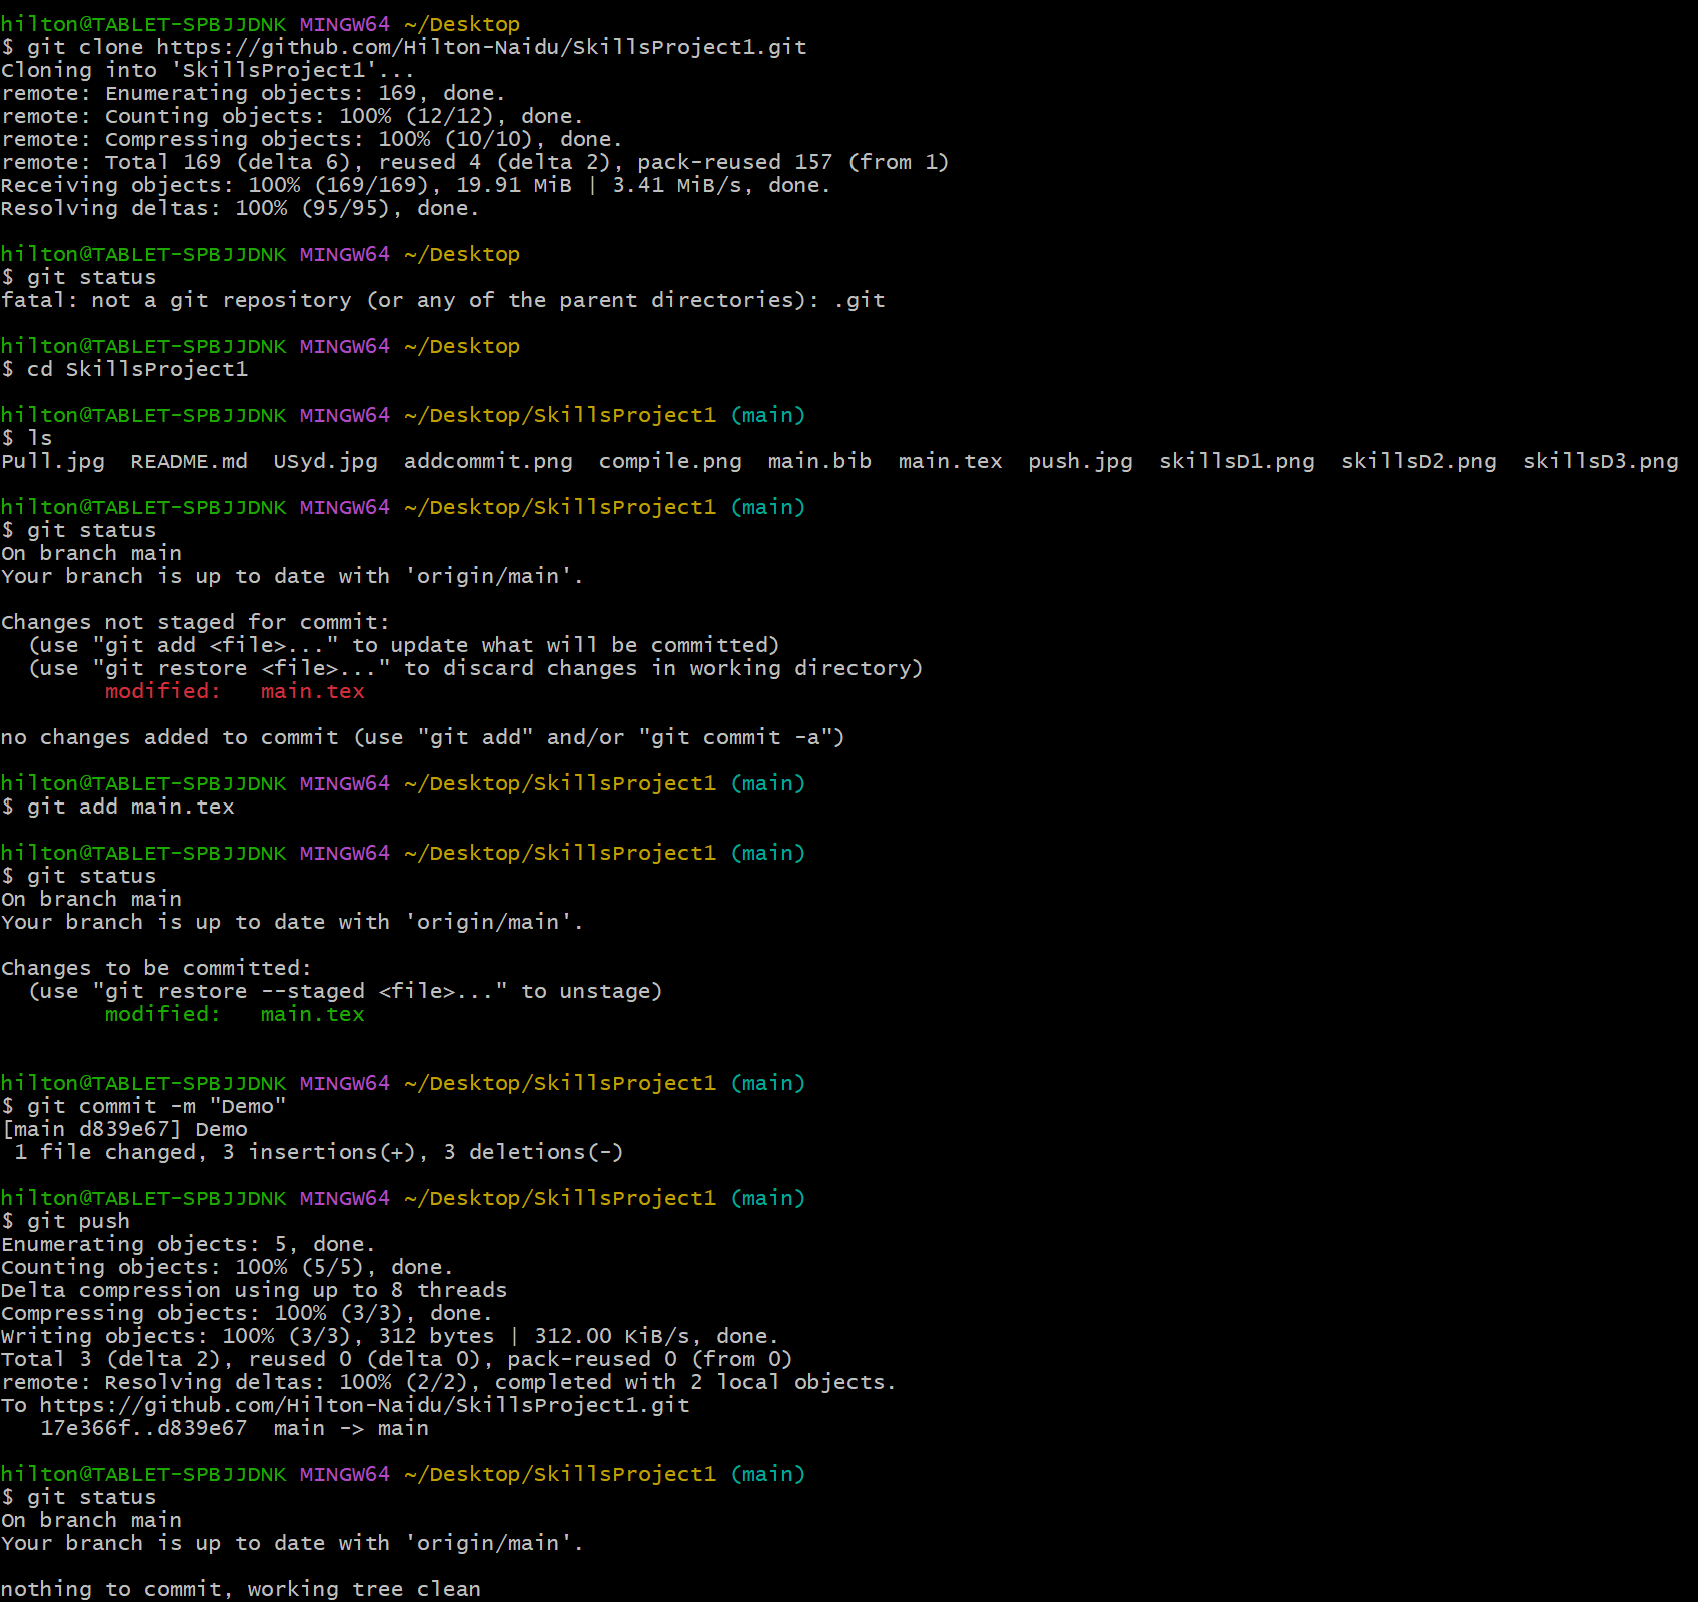
\includegraphics[width=6cm]{HiltonGit.png}
\caption*{(a) Git}
\end{minipage}%
\hfill
\begin{minipage}[t]{0.32\textwidth}
\centering
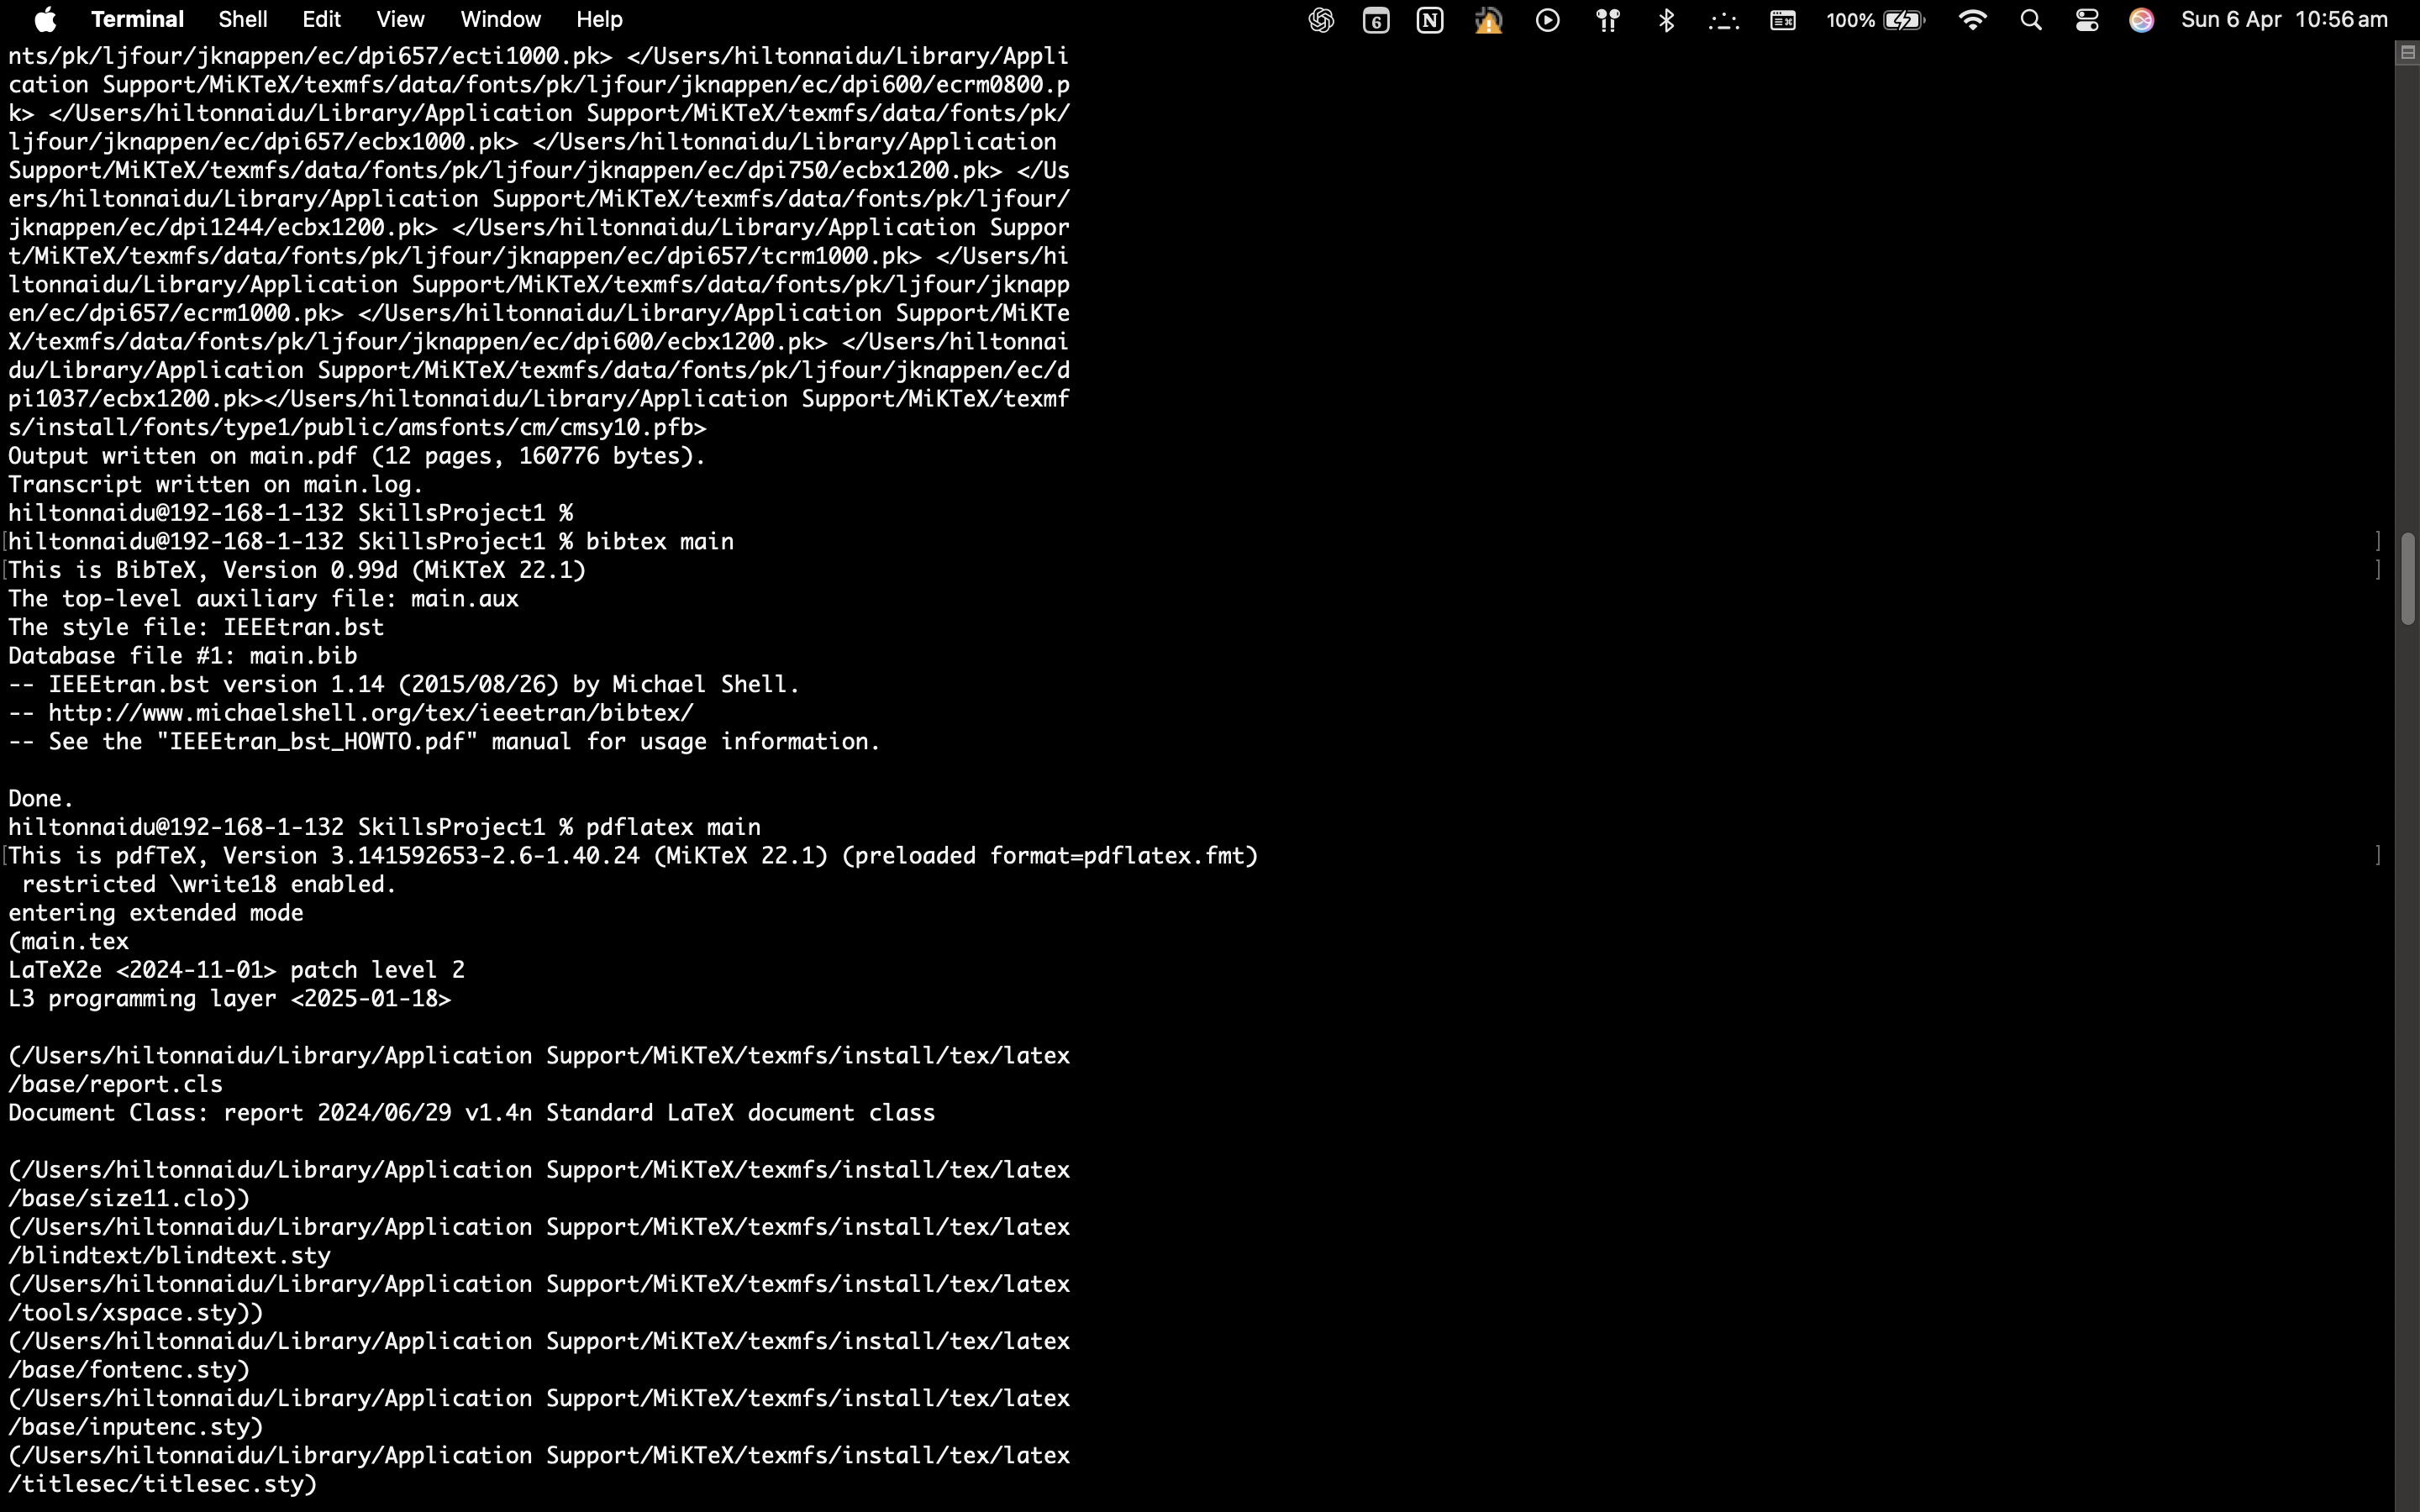
\includegraphics[width=6cm]{latexHilton1.png}
\caption*{(b) LaTeX 1}
\end{minipage}%
\hfill
\begin{minipage}[t]{0.32\textwidth}
\centering
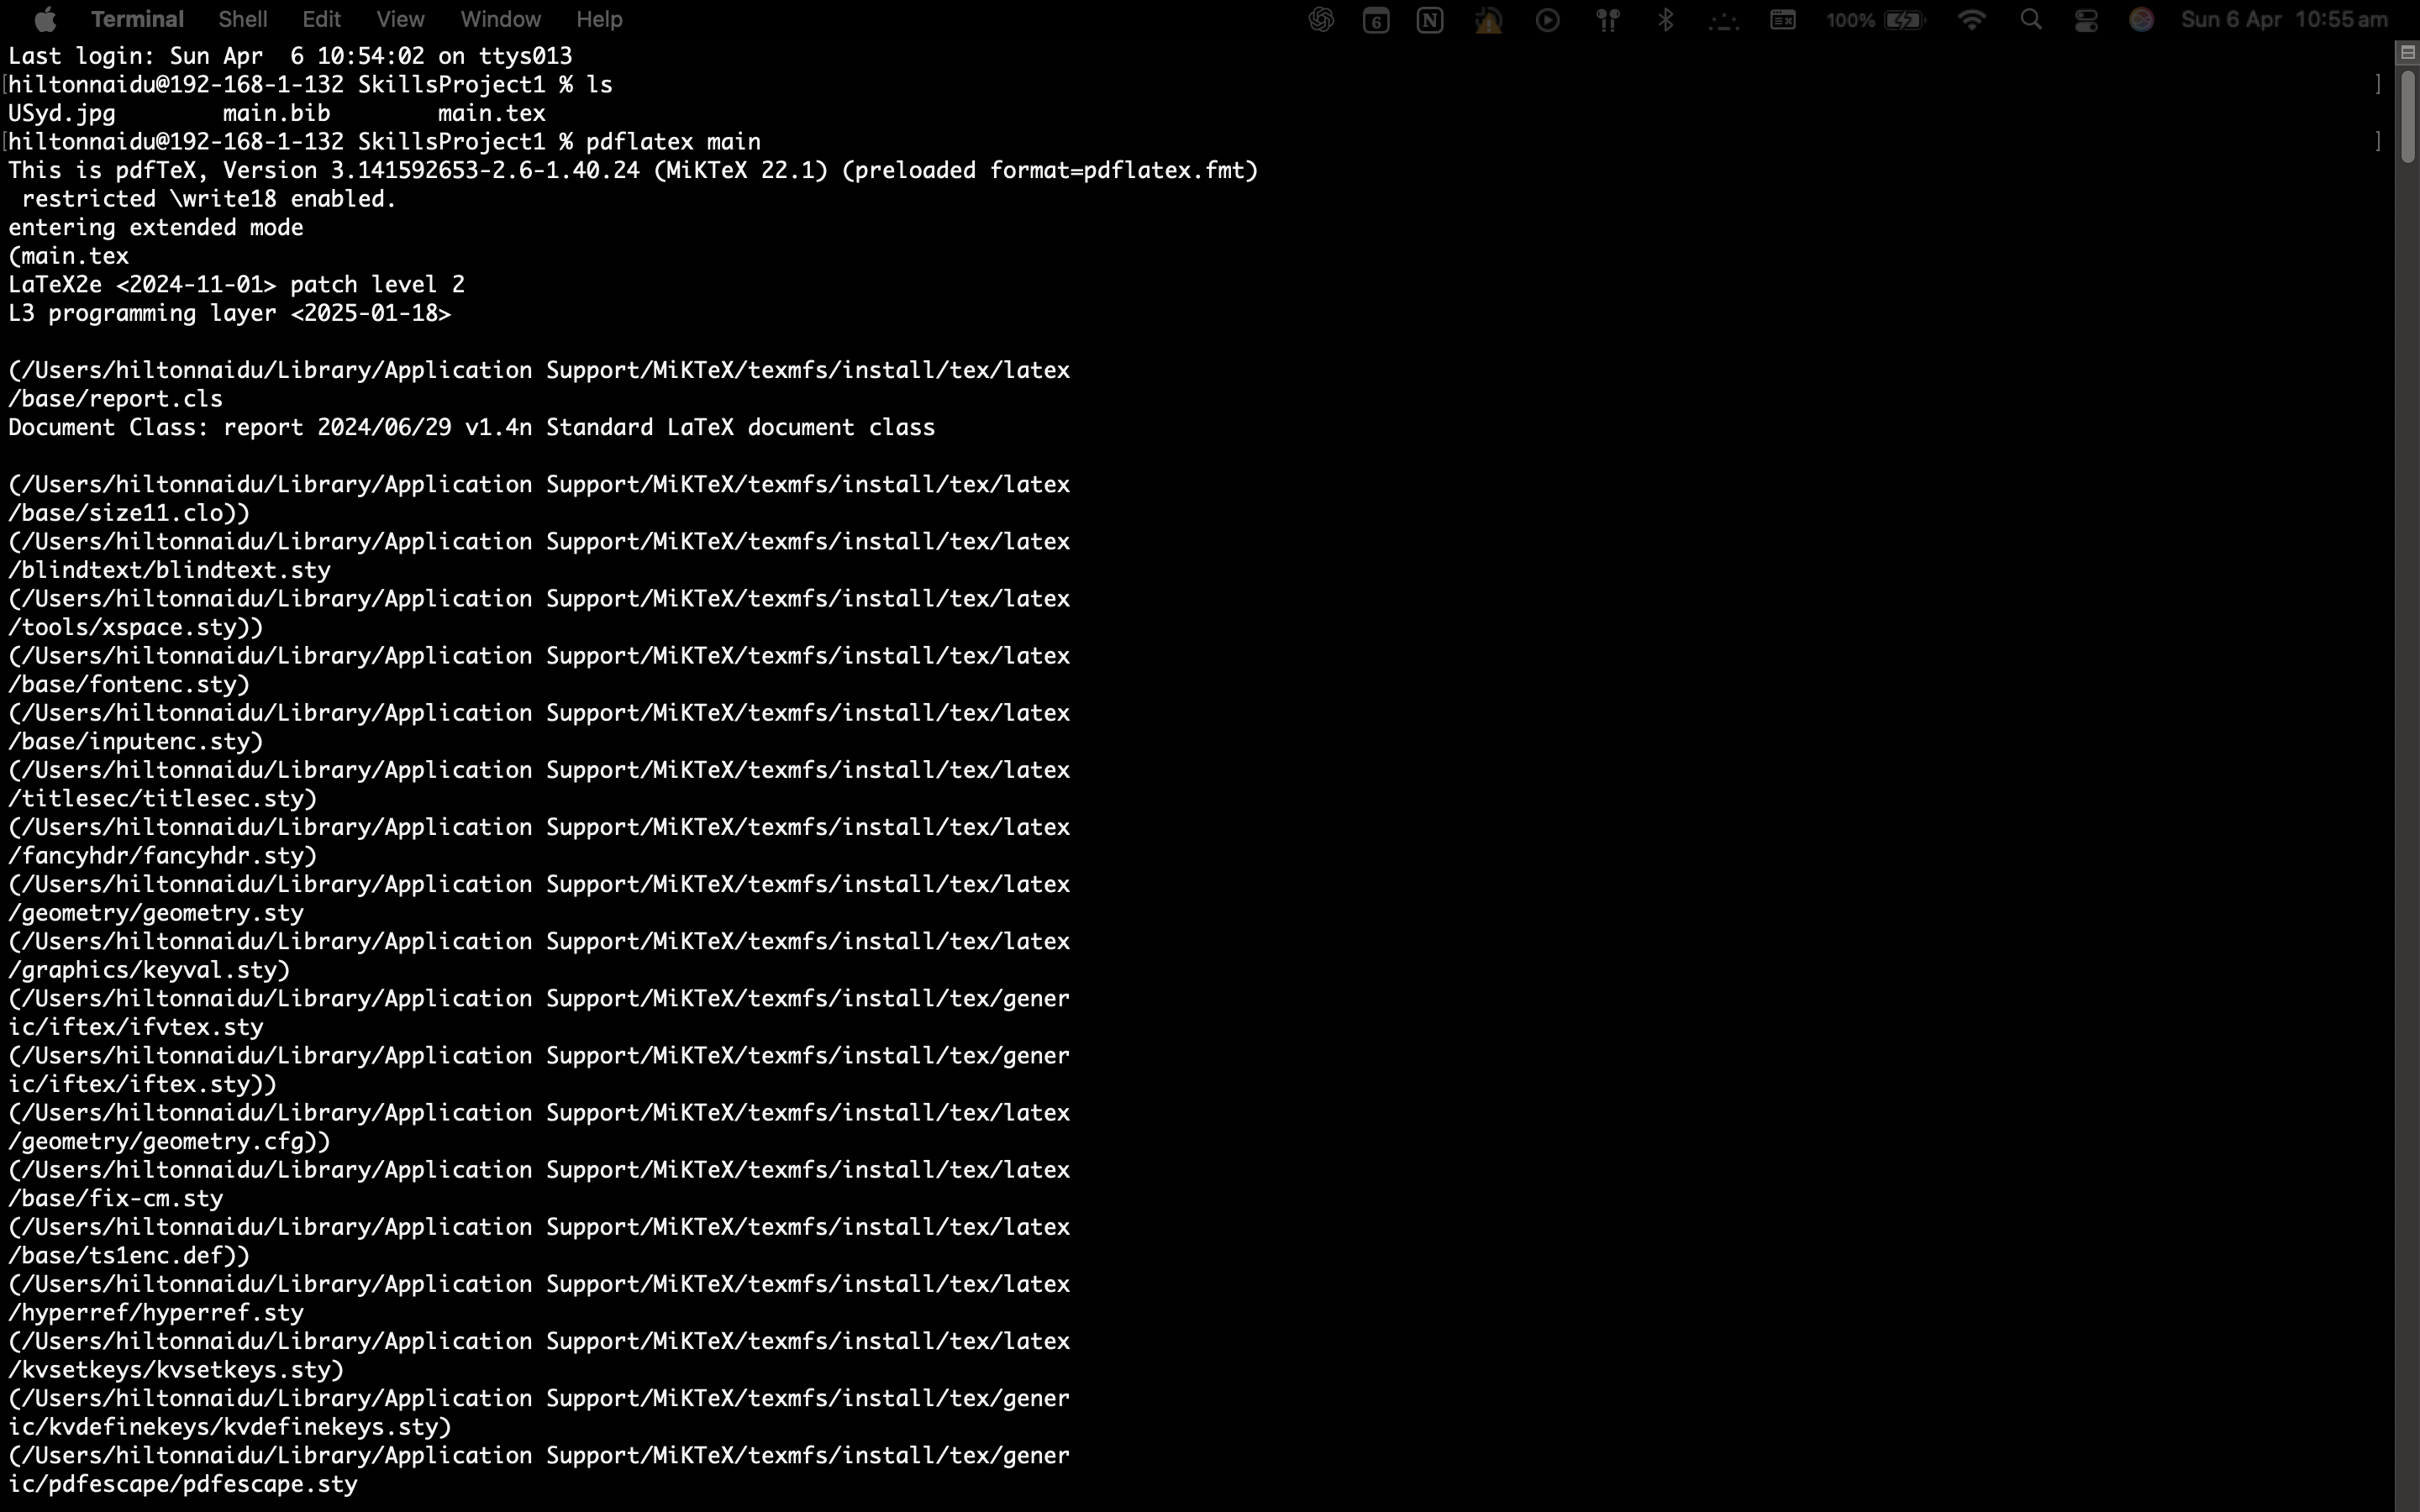
\includegraphics[width=6cm]{latexHilton2.png}
\caption*{(c) LaTeX 2}
\end{minipage}

\caption{Git and Latex terminal}
\end{figure}



\subsection{Skills for \majB: \studB}

To visualize natural disaster forecasts using historical and real-time data, identify high-risk areas, optimize emergency responses, and collaborate with computing professionals, the relevant SFIA 9 skills are:

\begin{enumerate}
	\item 1. Data analytics (DAAN): Enabling data-driven decision-making by extracting, analyzing, and communicating insights from structured and unstructured data \cite{palma2023}. In this project, DAAN plays an important role in predicting needs and providing the best solutions using past and real-time disaster data. It helps me analyze the given datasets, spot patterns, and share useful insights. Using data analytics, I can help decision-makers predict future trends, improve resource use, and make emergency responses more effective during natural disasters.


	\item 2. Data science (DATS): Applying mathematics, statistics, data mining, and predictive modeling techniques to gain insights, predict behaviors, and generate value from data \cite{palma2023}. In this project, DATS supports DAAN by using advanced methods, machine learning, and algorithms to analyze disaster-related data. As a data scientist, using DATS techniques helps me find deeper insights, create predictive models, and make decisions in real time that DAAN can use to improve forecasts and responses. DATS also helps build models that predict disaster patterns, which are important for planning needs and ensuring effective emergency responses. It is a key part of DAAN, as it provides the foundation for making data-driven decisions \cite{anderson2008}.
\end{enumerate}

	Collaborating with peers broadens my perspective and helps improve my DATS skills. Their feedback strengthens my coding, modeling, and analytical abilities. When I struggle with identifying relationships in the data or encounter errors I can't debug, explaining the issue to teammates often clarifies my thoughts. Sometimes, the explanation alone helps me gain new insights and solidify my understanding of the data. This collaborative process not only sharpens my skills but also enhances my ability to use DAAN for data-driven decision-making and problem-solving in complex situations by absorbing different opinions.

	During the team project, I identified that the most important skill I need to develop is Data Science (DATS). Throughout the assignment, I faced challenges in applying mathematical solutions to the data, and it made forecasting particularly difficult for me. To address this, I plan to improve my mathematical skills and focus on solving data-related problems to enhance my ability to analyze and forecast effectively. Strengthening this skill will enable me to make better data-driven decisions and improve my overall performance in future data science projects.
Strong Demo


\begin{figure}[htbp]
\centering
\begin{minipage}[t]{0.48\textwidth}
\centering
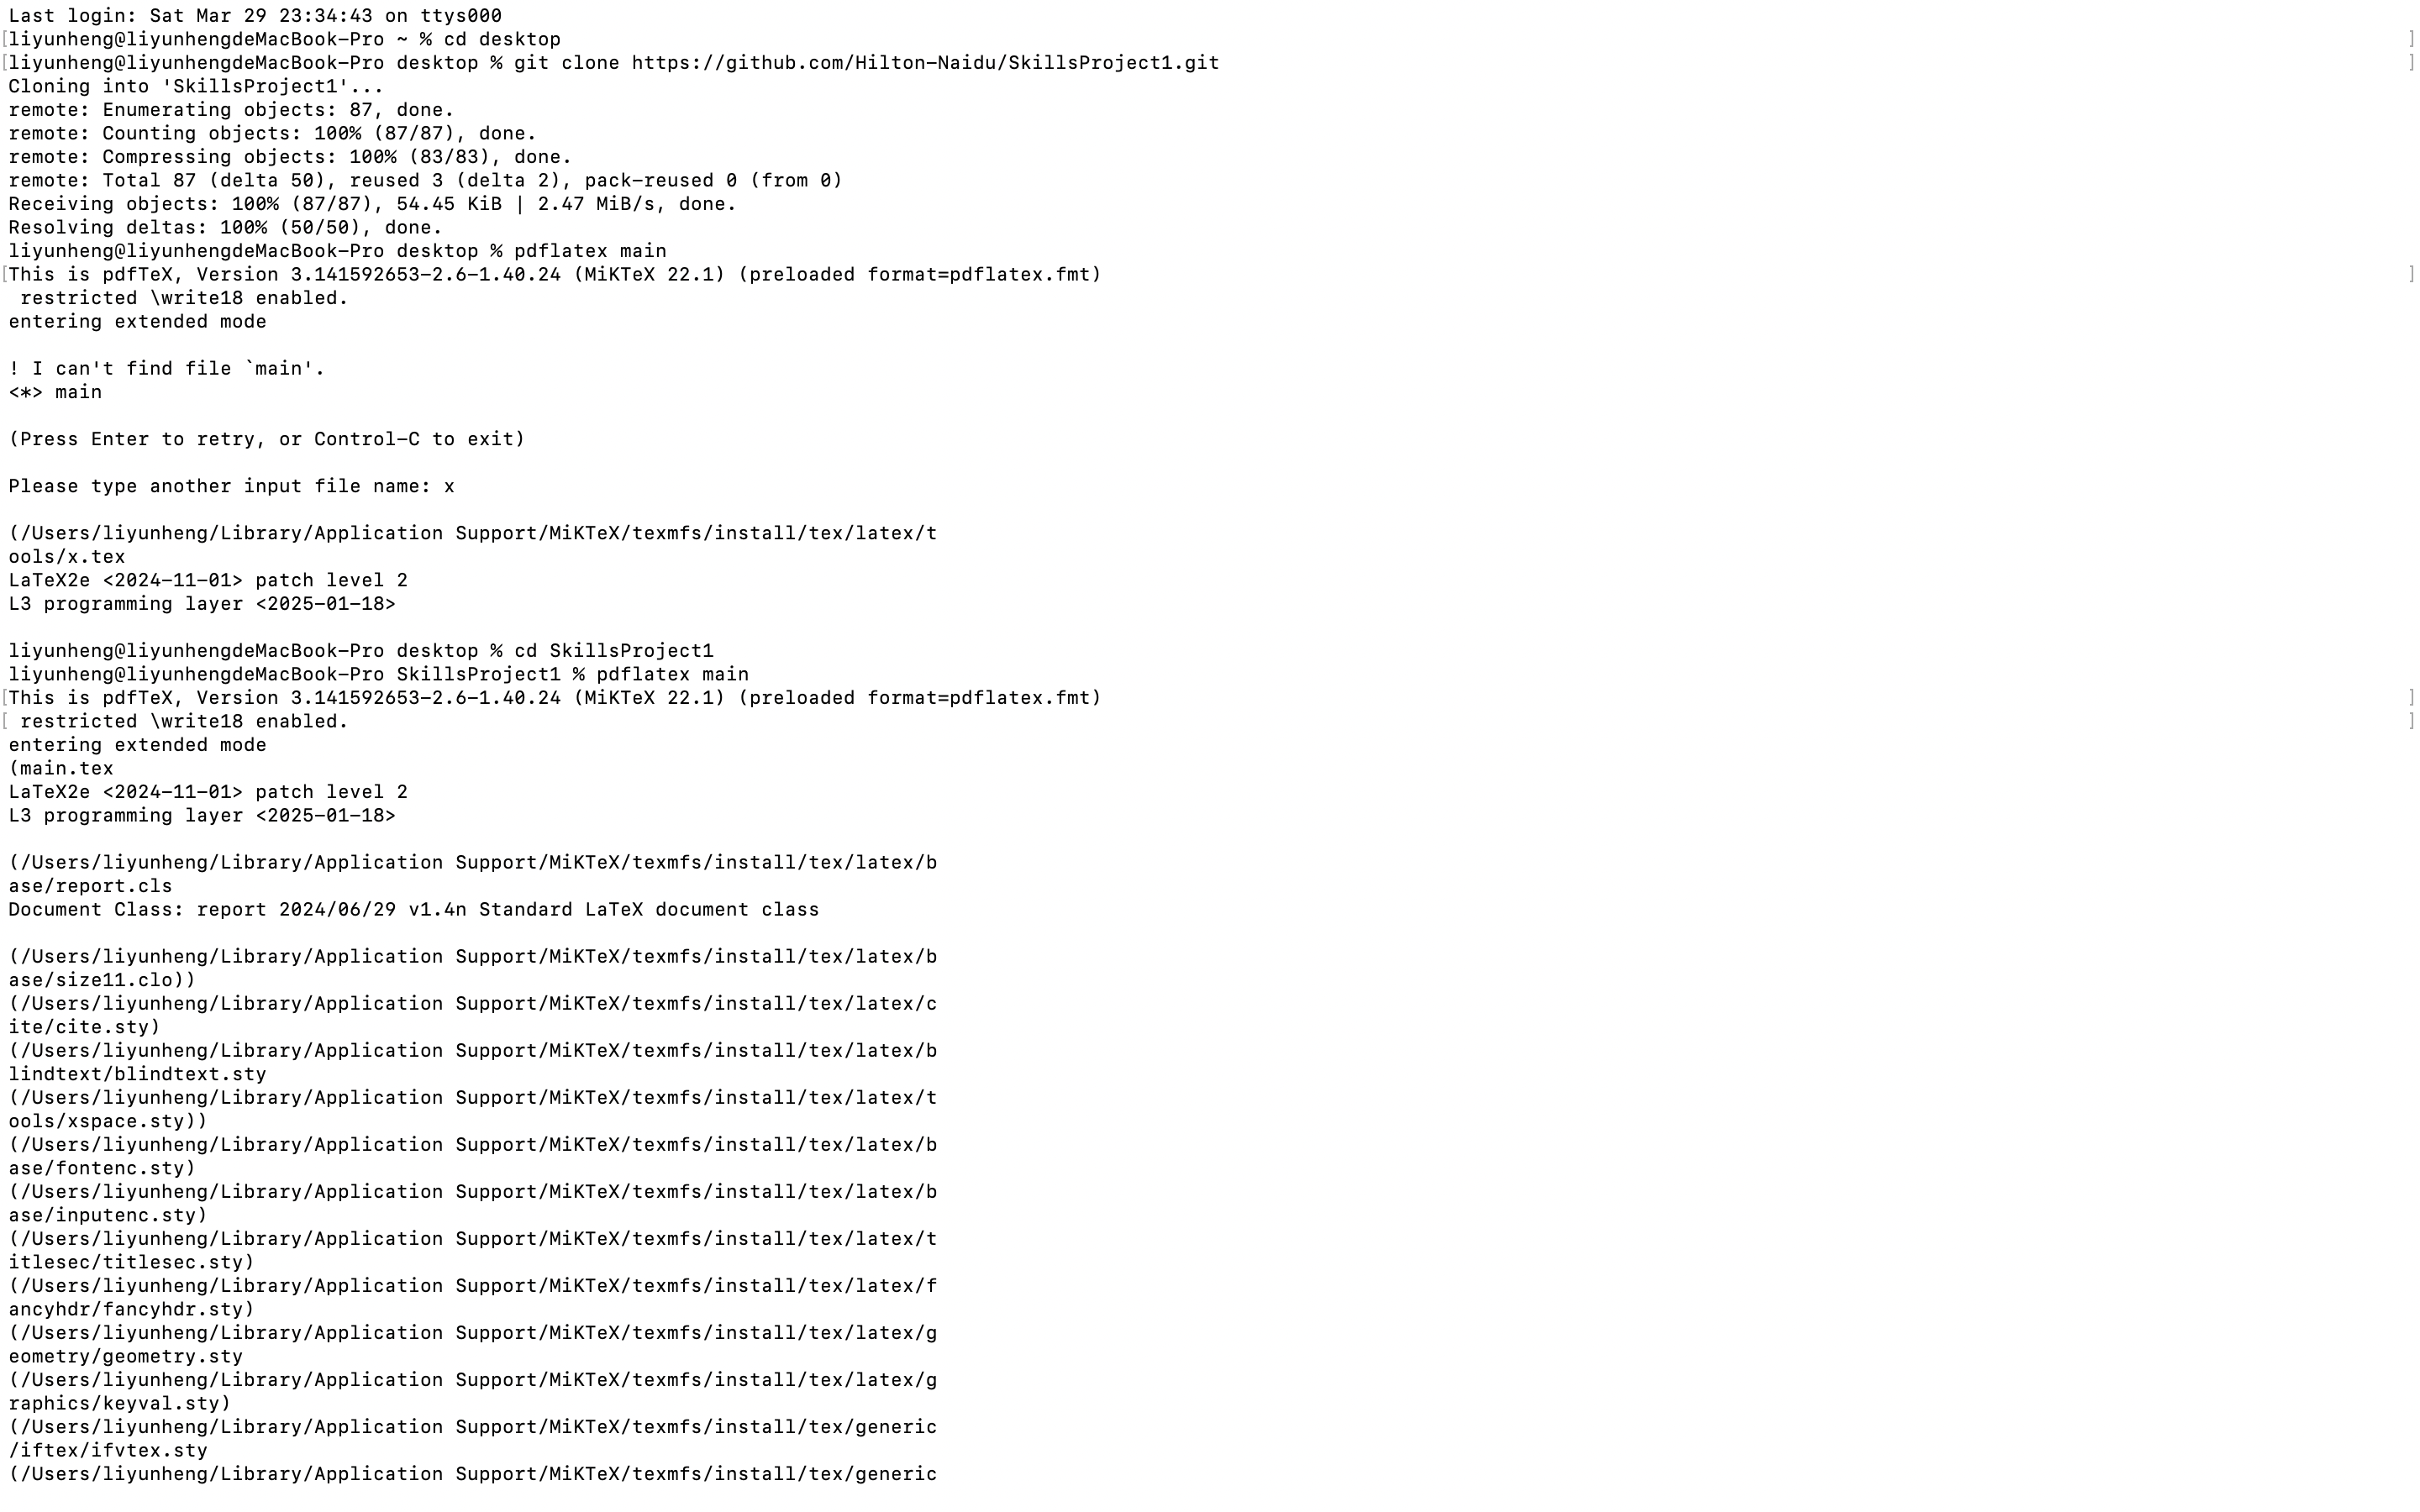
\includegraphics[width=6cm]{compile.png}
\caption{compile}
\end{minipage}
\begin{minipage}[t]{0.48\textwidth}
\centering
\includegraphics[width=6cm]{pull.jpg}
\caption{pull}
\end{minipage}
\end{figure}

\begin{figure}[htbp]
\centering
\begin{minipage}[t]{0.48\textwidth}
\centering
\includegraphics[width=6cm]{addcommit.png}
\caption{add and commit}
\end{minipage}
\begin{minipage}[t]{0.48\textwidth}
\centering
\includegraphics[width=6cm]{push.jpg}
\caption{push}
\end{minipage}
\end{figure}
\clearpage






\subsection{Skills for \majC: \studC}

The relevant skills of the Software Engineer are to "ensure a scalable, efficient, robust, user-friendly infrastructure with offline capabilities to manage disaster response and amount of people affected." The relevant SFIA areas are:
\begin{enumerate}
	\item Infrastructure Design (IFDN): Designing technology infrastructure to meet business requirements, ensuring scalability, reliability, security and alignment with strategic objectives \cite{palma2023}. In this project, IFDN plays a primary role in ensuring an infrastructure that can manage the unpredictability of material disasters that are common occurrences during natural disasters. Therefore, designing offline capabilities is essential for the software engineer to maintain operations during telecommunication disruptions. Furthermore, a user-friendly design allows responders to interact with the system under pressure.
	\item Systems Integration (SINT): This involves planning, implementing and controlling activities to integrate system elements, subsystems and interfaces to create operational systems, products or services \cite{palma2023}. Building on infrastructure design, system integration ensures that different system components, such as databases, emergency services, and communication networks—work together seamlessly. In this project, SINT is critical in highlighting how different subsystems (offline capabilities) would interact to ensure the system functions normally and without any bugs. This involved planning how different systems interacted (data systems, emergency responses, user interfaces) to form a cohesive structure. Since there was no coding, this is more about planning how the relationships in this system operate.
 \end{enumerate}

Working collaboratively on this project has strengthened my understanding of the core skills of a software engineer. Working in a group allowed us to share our own unique views on our differing roles and what we do, helping clarify to me what my title entails. It helped me improve my analytical skills, portraying how breaking down a large task into smaller subcomponents can help more clearly show how to best go about a project. Collaborating in a group helped me better understand the interconnectedness between various system components and how they must function together to ensure functionality. Furthermore, my group members' consistent feedback assists by providing a unique understanding of the project.

I recognised that communication was paramount in this group project and was an evident skill that I need to improve; this aspect extends to all group projects. While I actively participated in discussions and contributed to group collaboration, I recognised that I could have been more active within the group, helping organise meeting locations and times. Furthermore, doing more personal work before coming to group discussions helps with easily communicating our independent roles and thus allows us to best approach group issues.

\newpage
\begin{figure}[htbp]
\centering
\begin{minipage}[t]{0.45\textwidth}
\centering
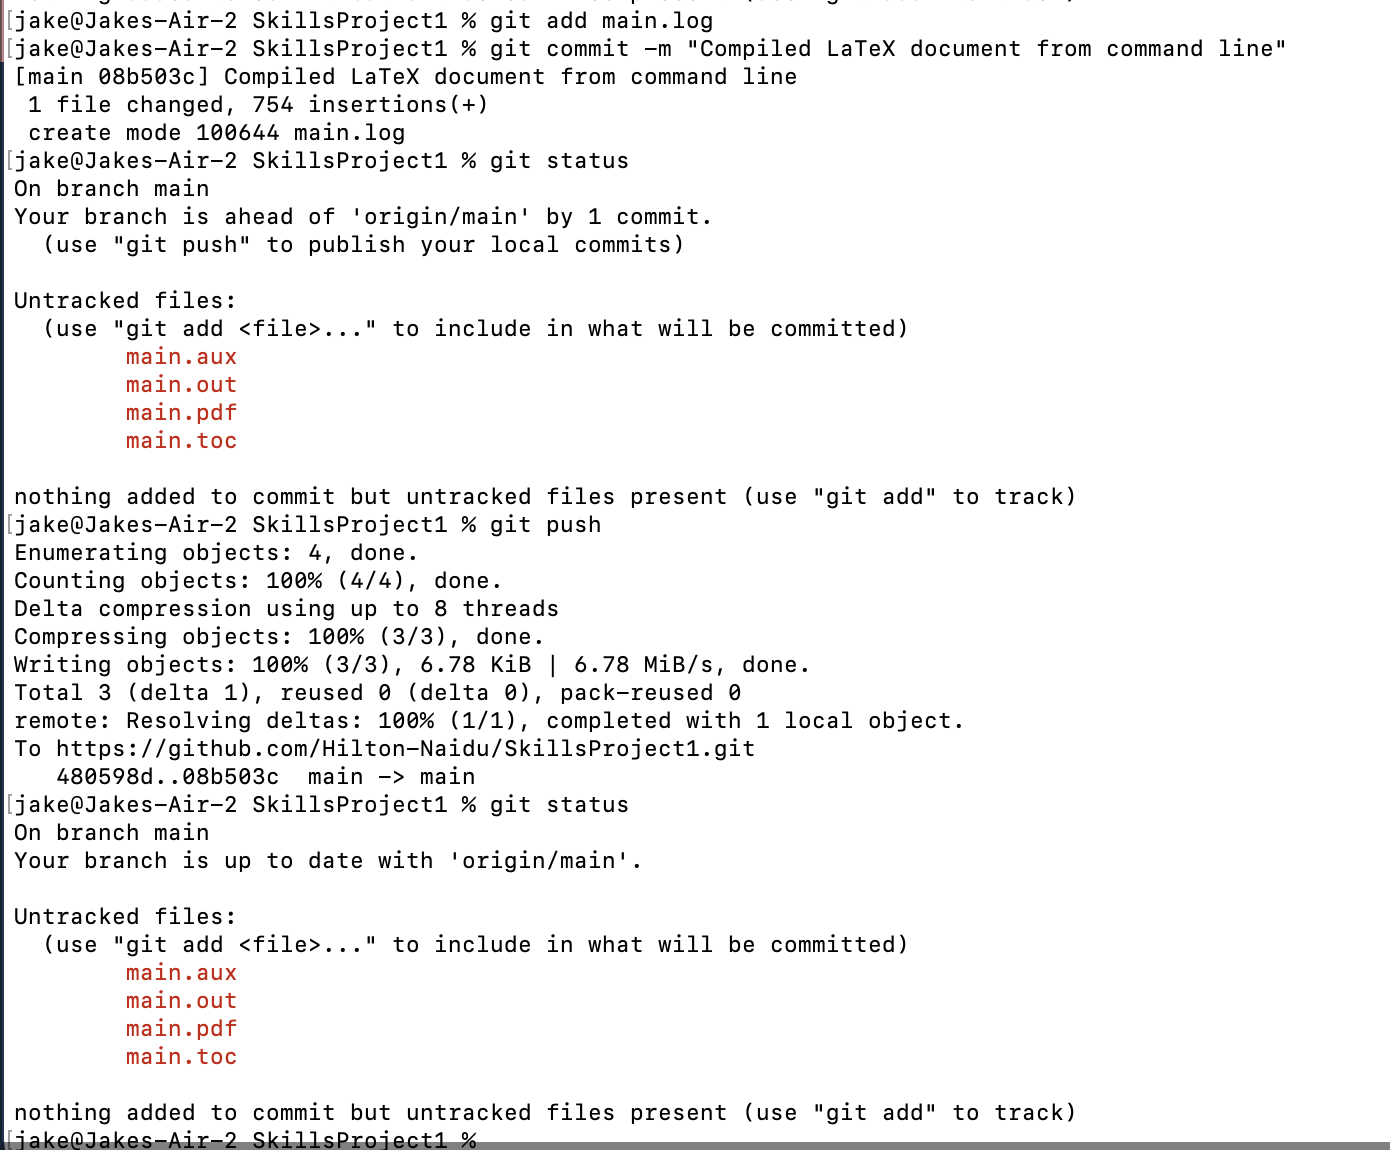
\includegraphics[width=\linewidth]{jakecommit.png}
\caption*{(a) Commit}
\end{minipage}
\hfill
\begin{minipage}[t]{0.45\textwidth}
\centering
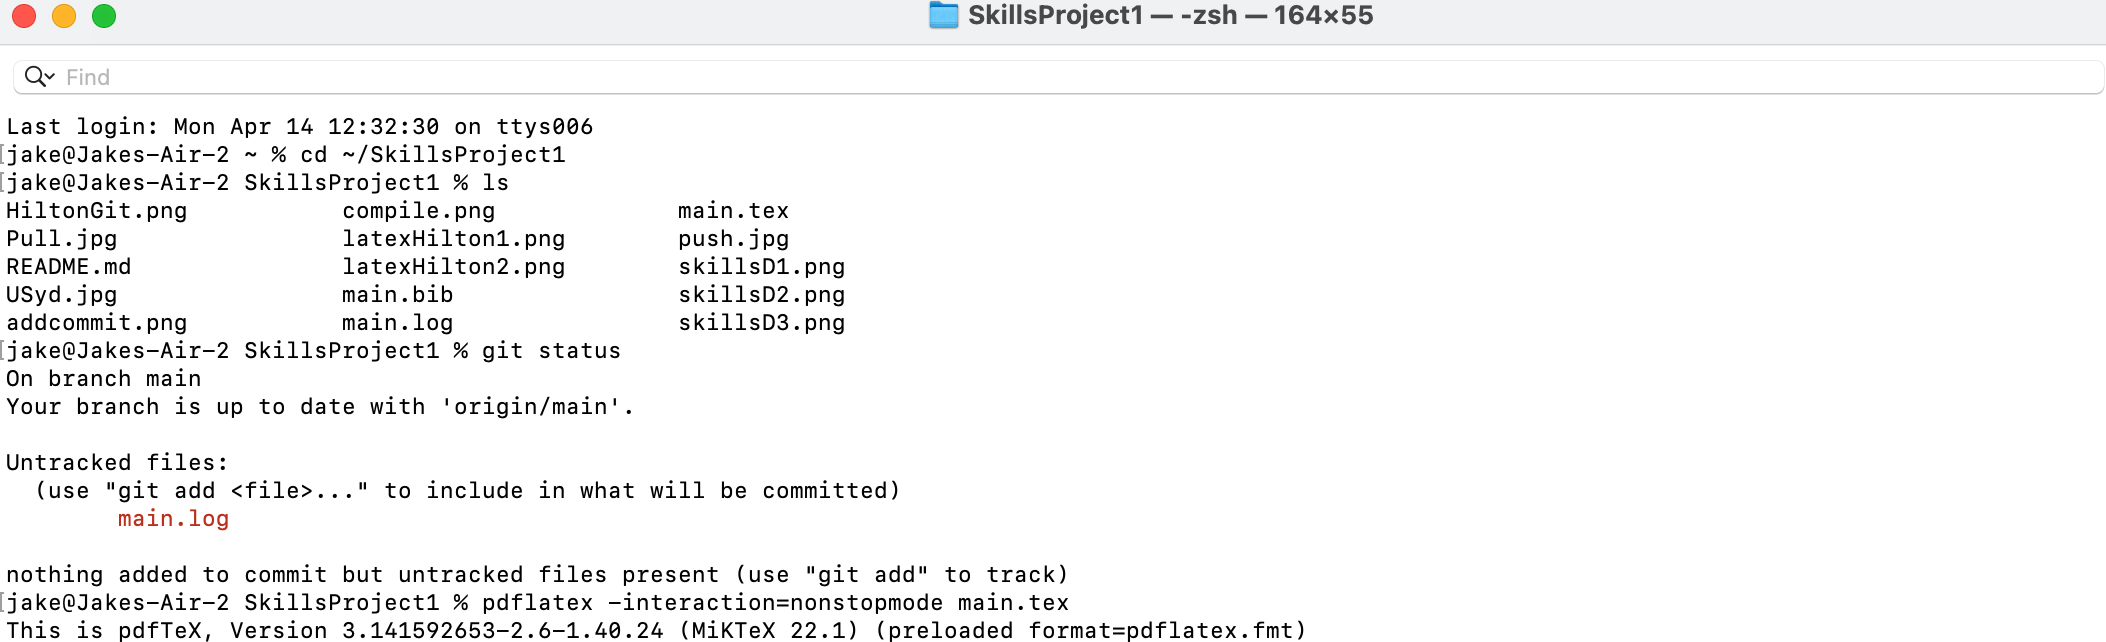
\includegraphics[width=\linewidth]{jakecompile1.png}
\caption*{(b) Compile 1}
\end{minipage}

\vspace{0.5cm}

\begin{minipage}[t]{0.45\textwidth}
\centering
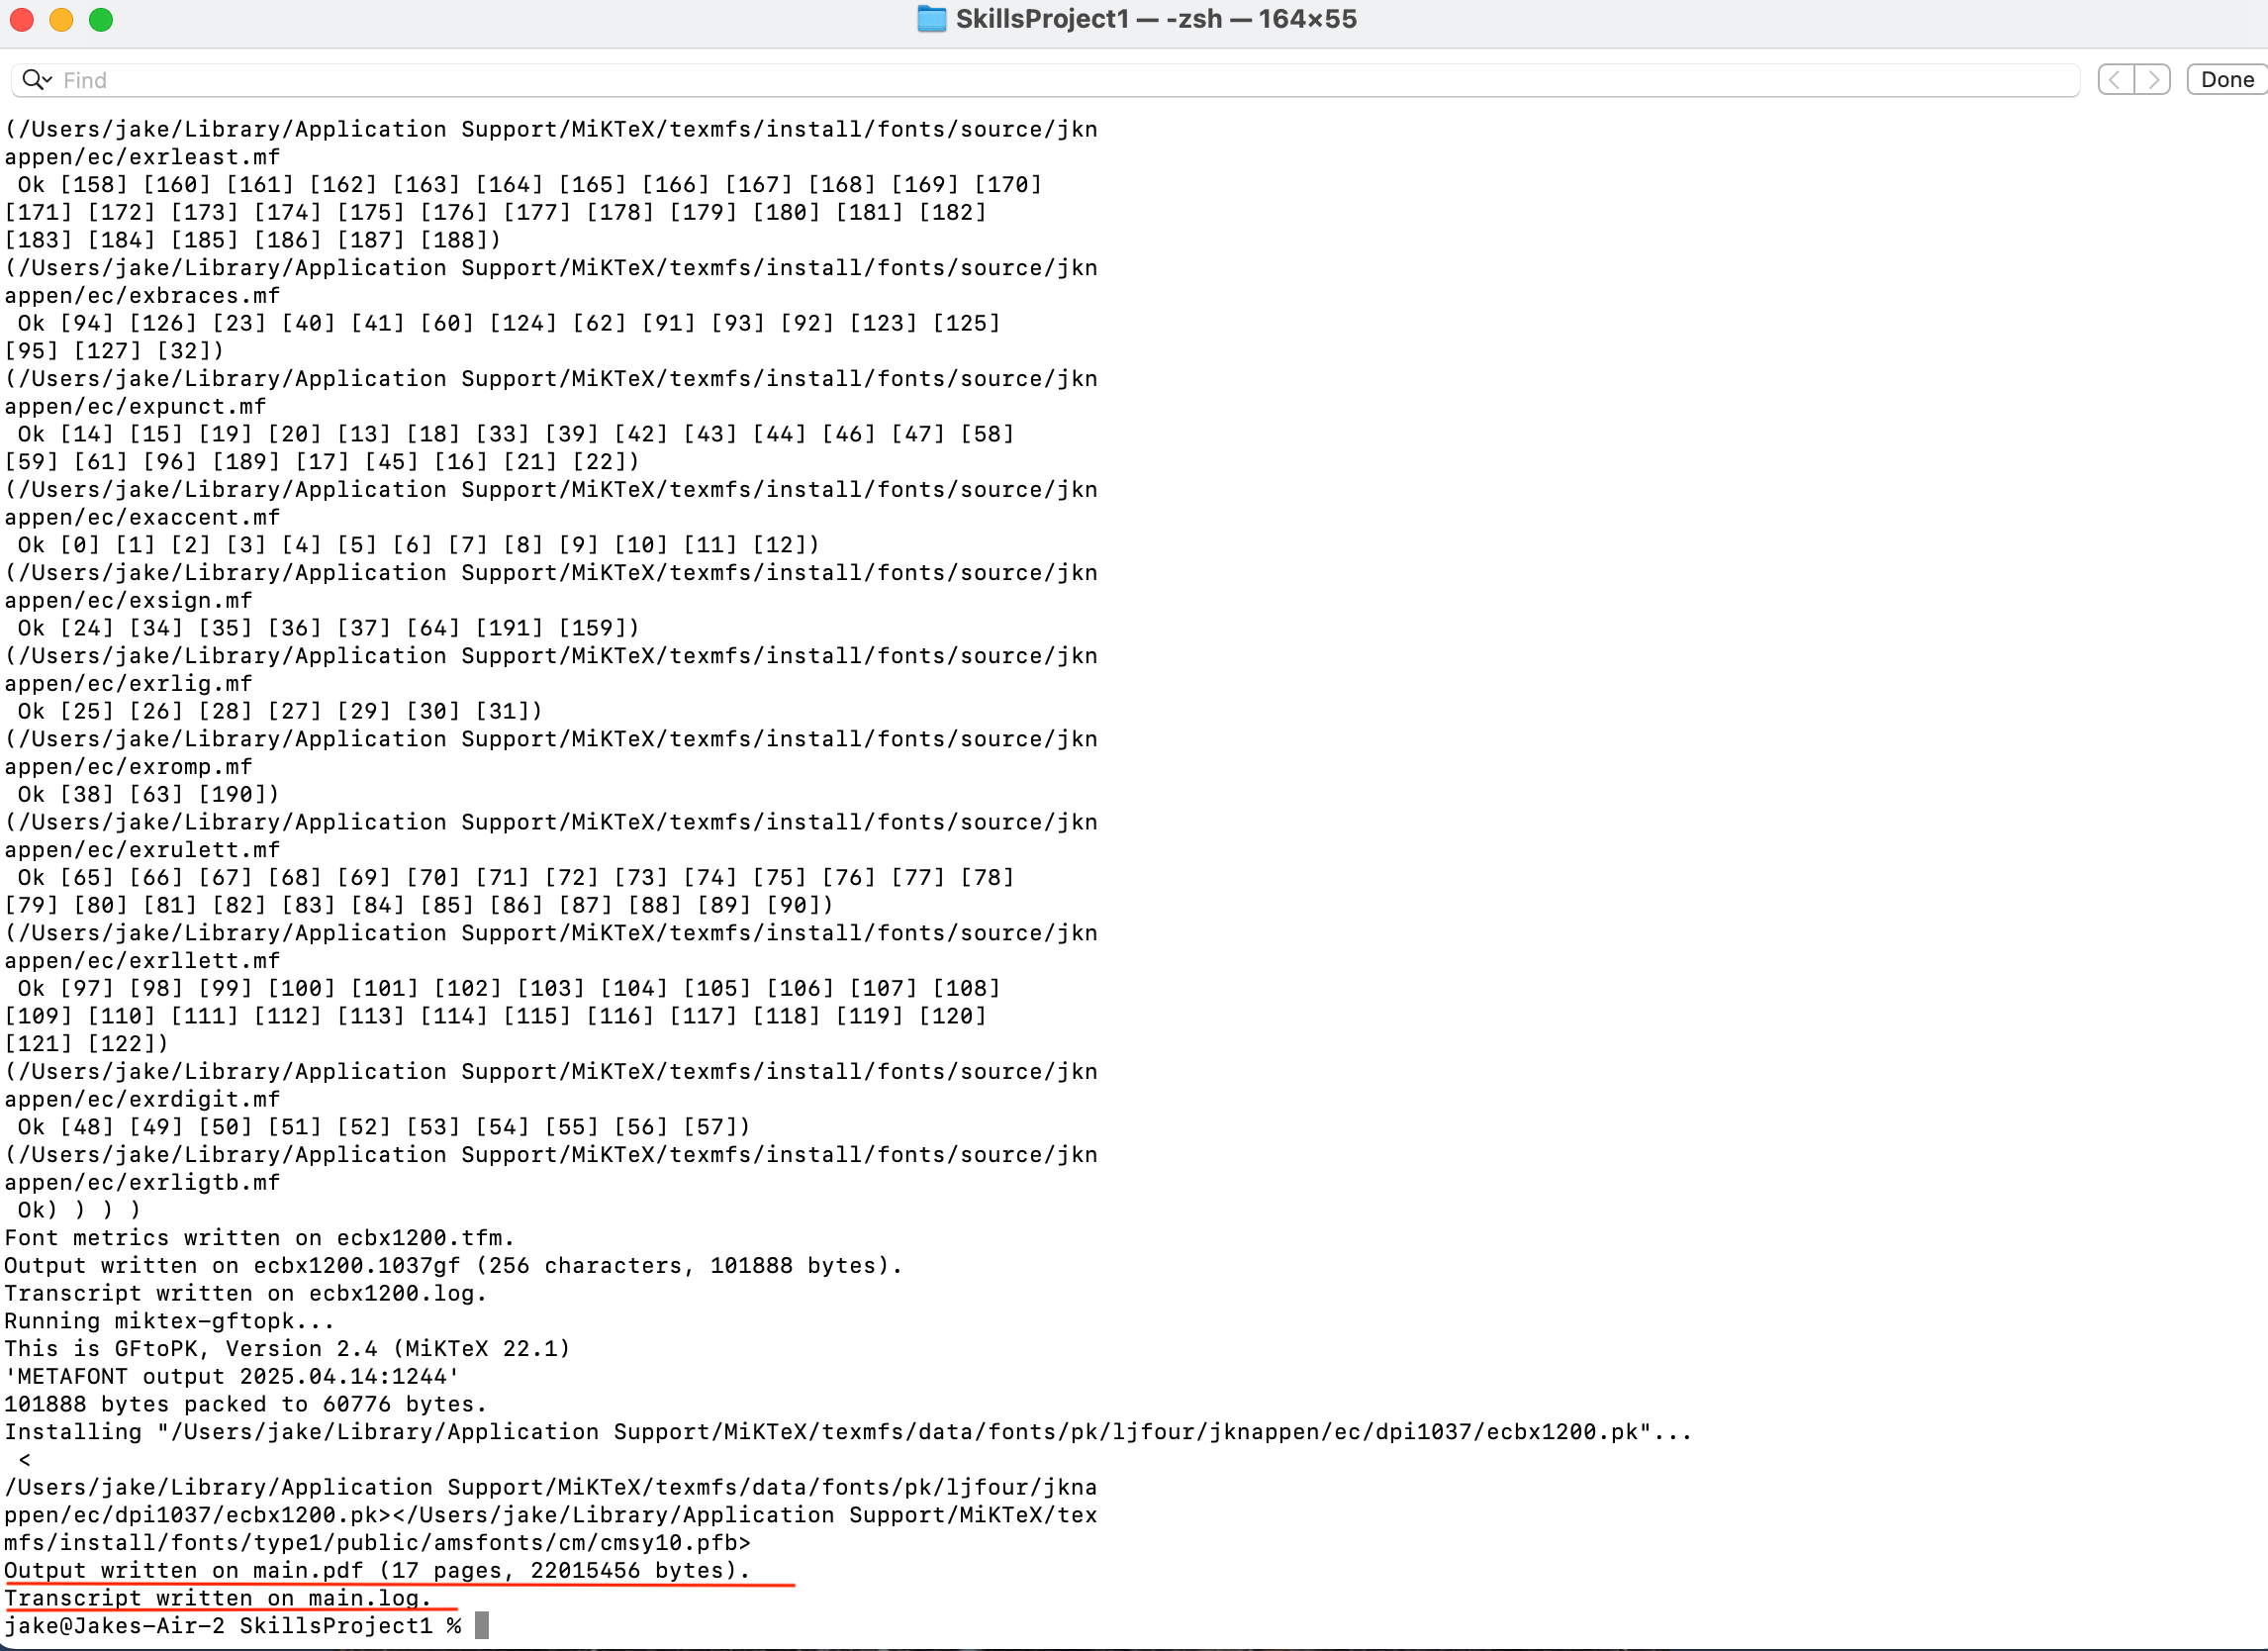
\includegraphics[width=\linewidth]{jakecompile2.png}
\caption*{(c) Compile 2}
\end{minipage}
\hfill
\begin{minipage}[t]{0.45\textwidth}
\centering
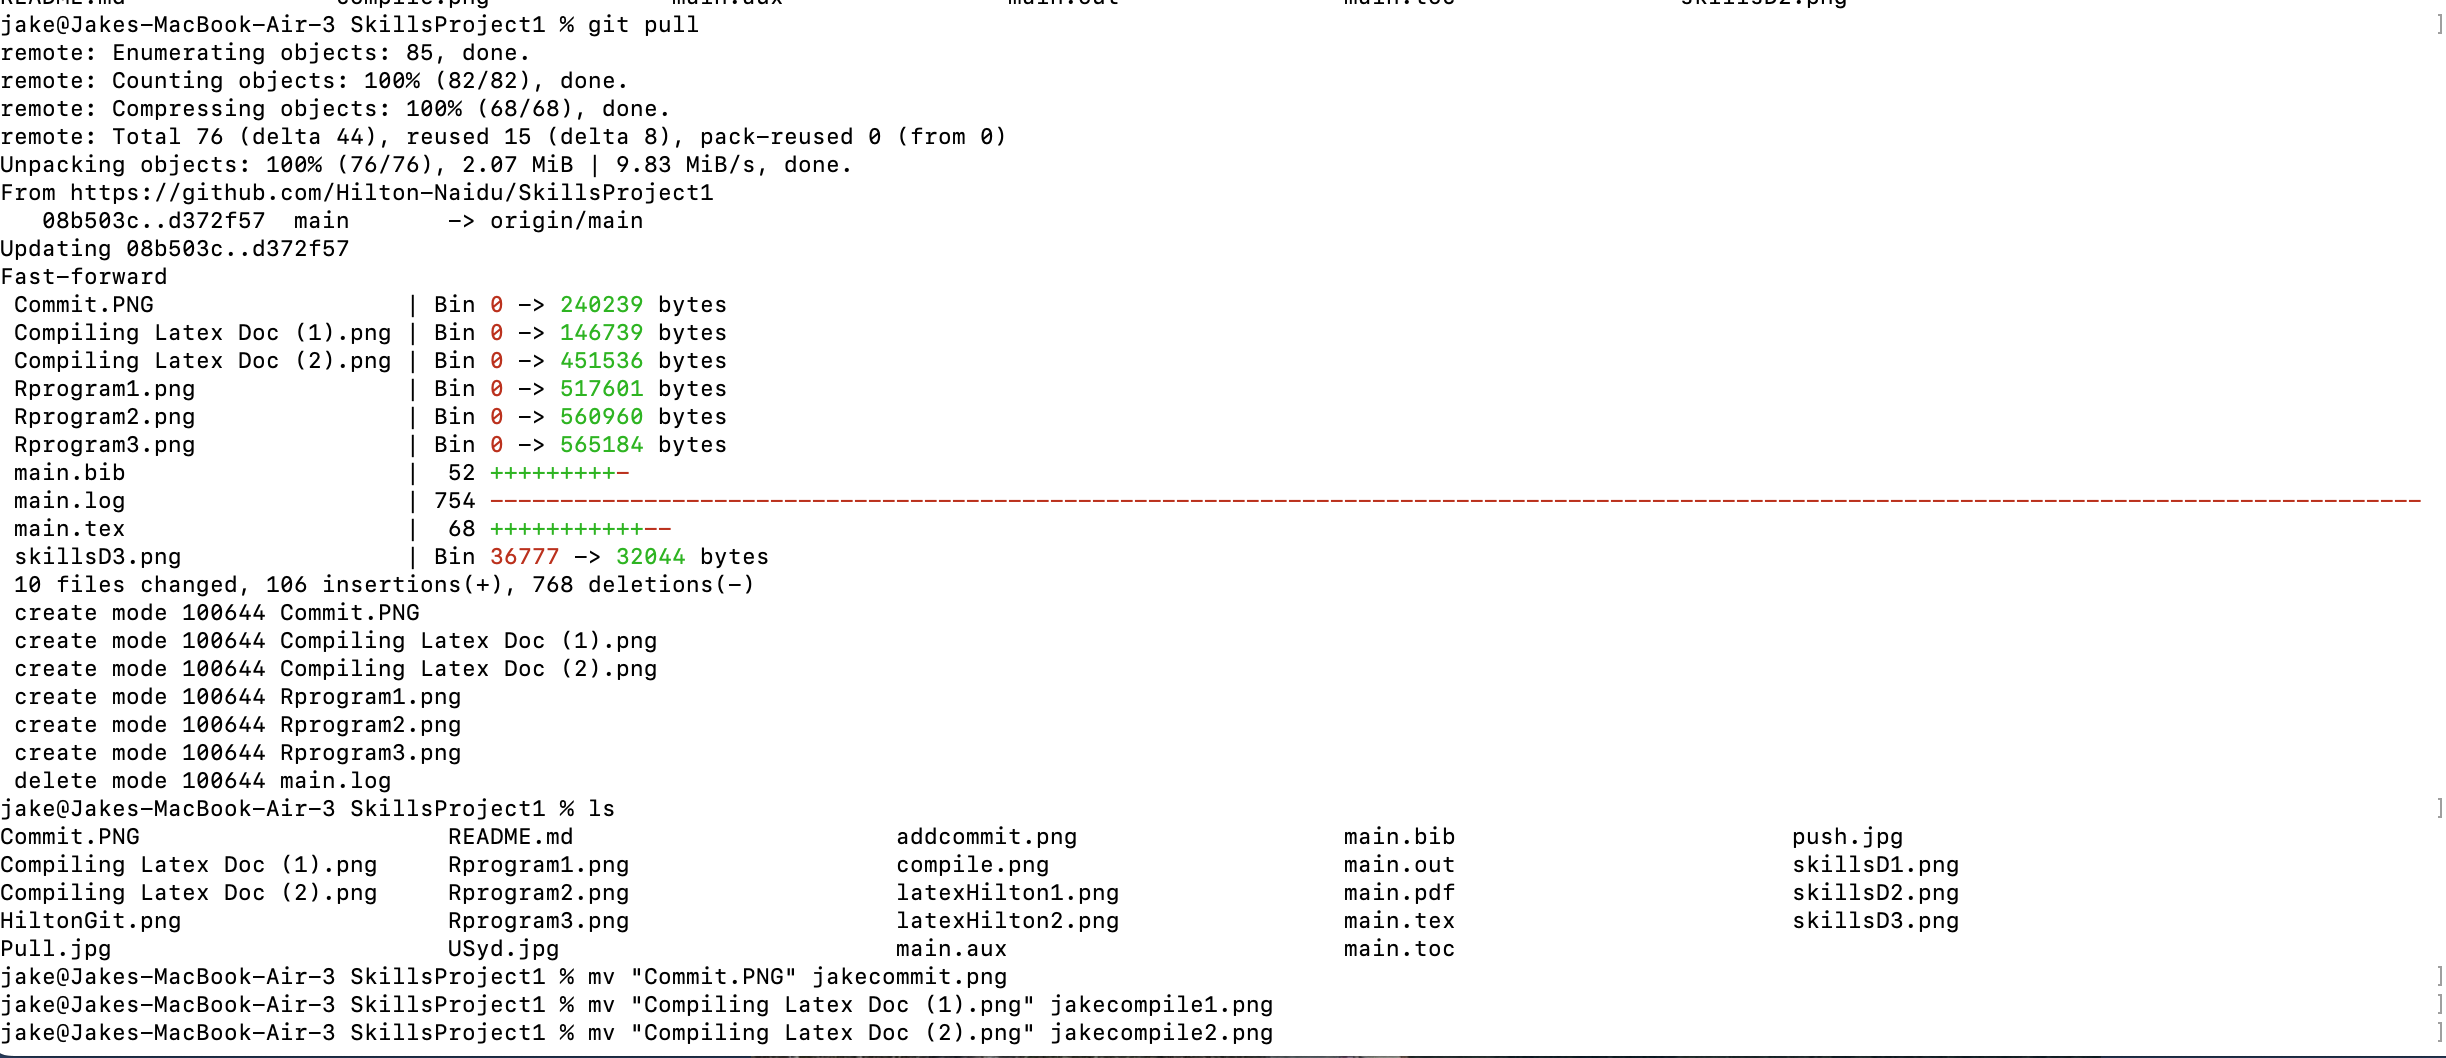
\includegraphics[width=\linewidth]{jakepull.png}
\caption*{(d) Pull}
\end{minipage}

\caption{My Git and LaTeX workflow steps}
\end{figure}
\clearpage

\subsection{Skills for \majD: \studD}

The 2 most relevant SFIA 9 skills \cite{sfia} for a cybersecurity specialist working in the industry to protect the safety and privacy of digital systems and data is as follows:

\begin{enumerate}

	\item Information Security (SCTY): This skill involves managing and developing security controls and management strategies \cite{scty}. The development and maintenance of an effective information security strategy that aligns with the organization's overall goals is a vital skill in the cybersecurity industry. A well-integrated security approach enhances the protection of data and infrastructure without impeding overall operations. In this project, SCTY is an important skill for developing security infrastructures and strategies ensure that communication lines are maintained and the data is protected.

	\item Vulnerability Assessment (VUAS): THis skill involves identifying, classifying, and managing vulnerabilities in a system \cite{vuas}. Analyzing security vulnerabilities and business impact analysis to detect and mitigate the repercussions of security flaws ensures the solidity of data structures. In this project, VAUS plays a role in assisting SCTY by allowing security gaps to be fixed proactively to create a secure system that maintains its integrity even in critical situations by staying up to date with prevention strategies as well as keeping the team informed on threats and malicious actors \cite{papatsaroucha2021}.
\end{enumerate}

Working collaboratively on this project has helped greatly in strengthening the aforementioned skills. In particular, collaborating on this project has imporved my SCTY skills. By working in a team, I am exposed to a broader range of perspectives from different roles, ranging from analysts, developers, etc. These perspectives contribute to creating a comprehensive security system that is more intergrated with the overall operation. Working with my teammates to plan and devlelop the solution helps me better understand the overall structure of the project, allowing me to develop a solution that aligns more with the technical goals.

While working on this project, a skill I have identified to be further developed is Threat Intelligence (THIN). While working under a stressful and volatile situation such as managing an evolving natural disaster situation, the gathering and processing of threat information to adapt to new security concerns is important so that current measures are always up to date. I could have communicated more with other fields such as emergency responders to get a more comprehensive idea of the security threats I might face. Implementing an effective way to obtain new threat information as well as communicate the response strategy to all relevant parties will be a fruitful effort for future endeavors.

\begin{figure}
\centering
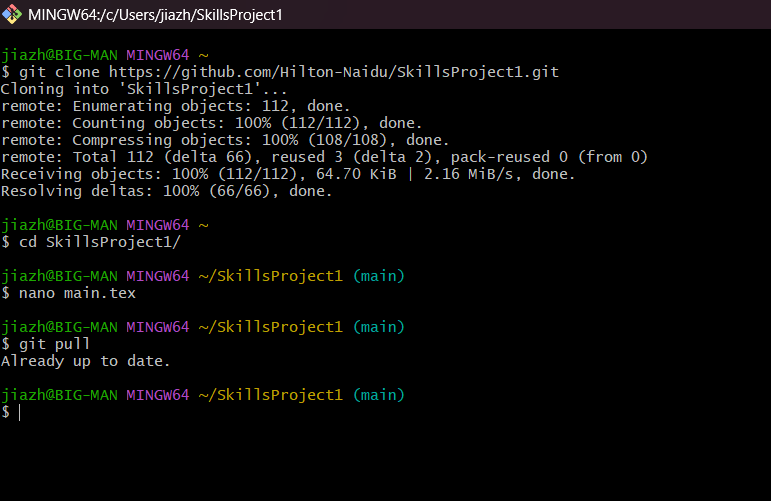
\includegraphics[width=0.75\textwidth]{skillsD1.png}
\caption{pulling from the git hub}

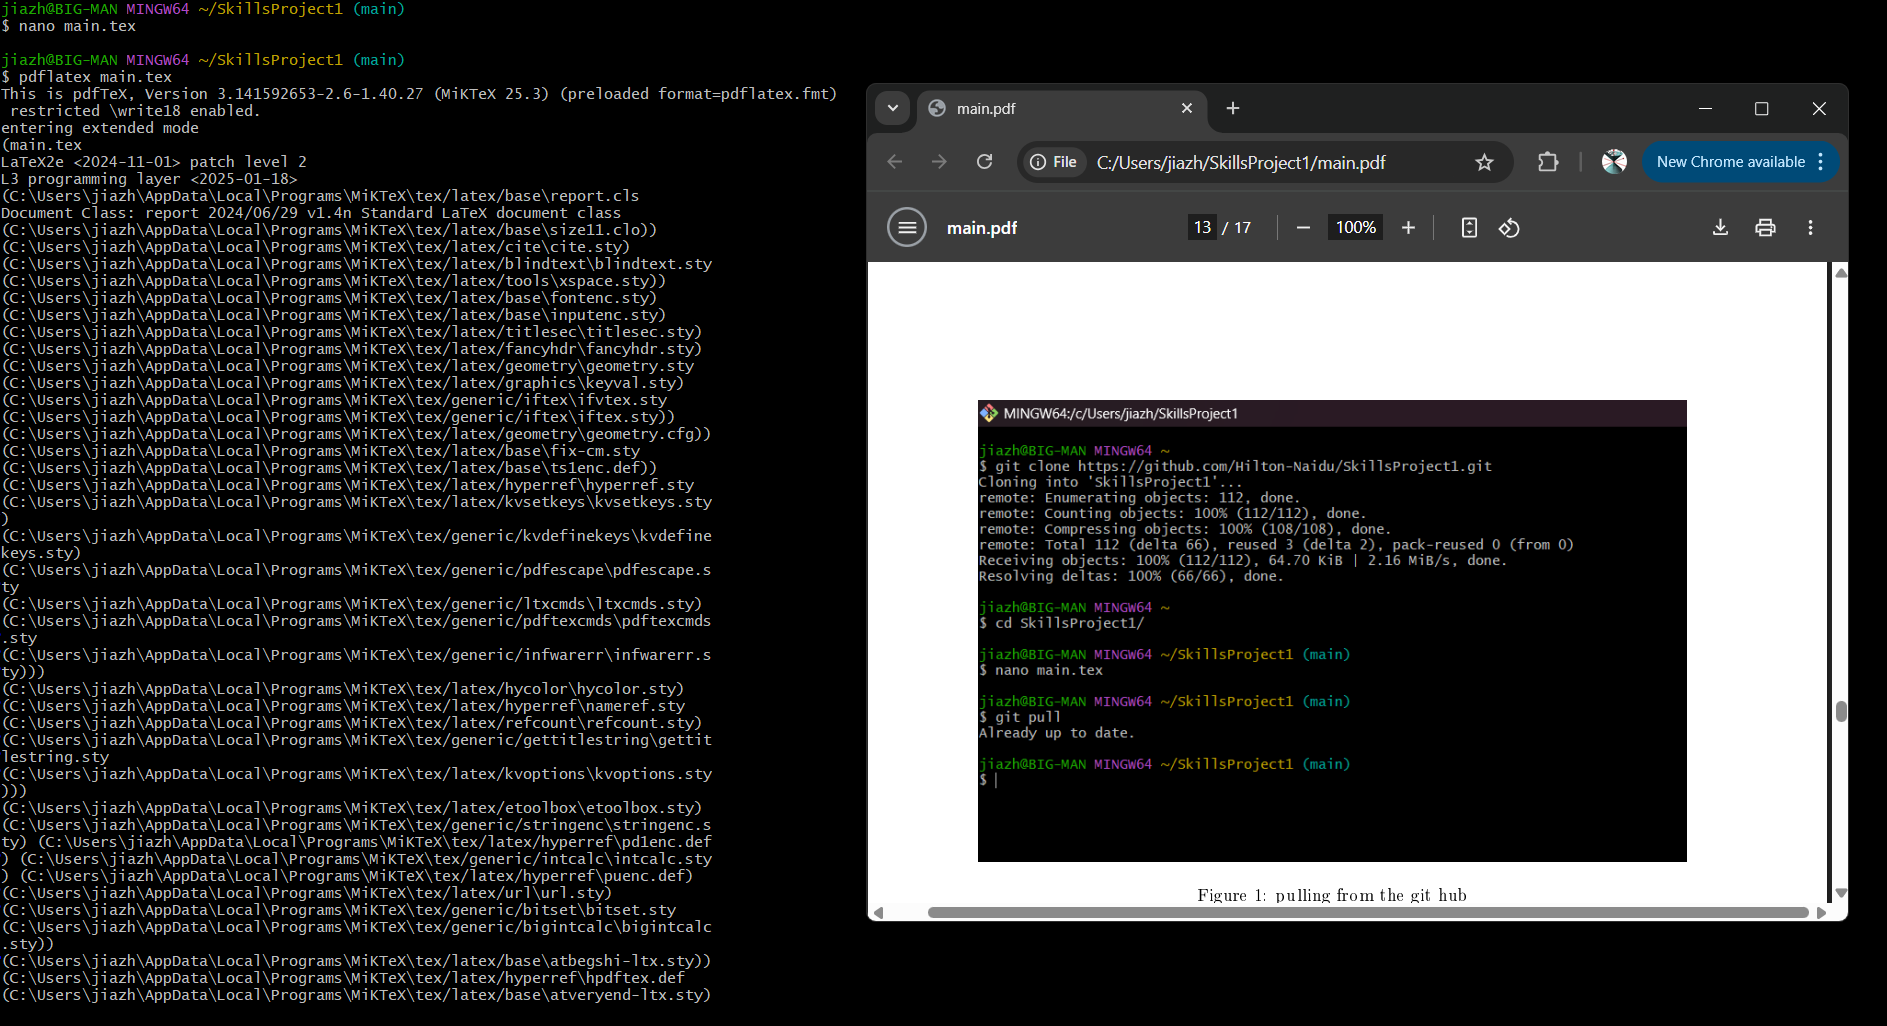
\includegraphics[width=0.75\textwidth]{skillsD2.png}
\caption{editing and recompiling the pdf}

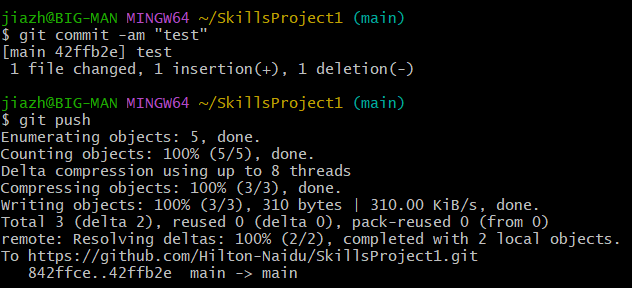
\includegraphics[width=0.75\textwidth]{skillsD3.png}
\caption{git commit and and git push}
\end{figure}

%add a fifth subsection if there is a fifth member

% ========================================================

\newpage
\section{Task 2 (Advanced): Advanced Skills}

Task 2 contains two components (both required).\\[2mm]

\textbf{Component 1: Project management}

The team is required to extend on your project on GitHub.

\begin{itemize}
    \item Add issues and assign as the project progresses
    \item Create parent issues and subdivide tasks into sub-issues
    \item Filter for fields in the project
    \item Create a line chart using GitHub project chart to represent project activity over time
\end{itemize} 

\vspace{4ex}

\textbf{Component 2: Exploration of Tech Tools}

This component focuses on researching and exploring industry-relevant tools within each domain and is split into 2 parts.

\vspace{2ex}


\textbf{Part A:}

Each student must undertake an exploratory analysis of the below tool relevant to their domain. 
Each student is to take on an exploration and investigative research of tools below relevant to their major. 

\begin{itemize}
    \item Computer Science: Python Websockets package (API requests and system integration)
    \item Data Science: choose between Python NumPy or Pandas package (data analytics)
    \item Cybersecurity: choose between Wireshark or Burp Suite (network security analysis)
    \item Software Engineering: choose between Python Pytest or UnitTest (software testing)
\end{itemize}
If there is a fifth member:
\begin{itemize}
    \item Human-Computer Interaction (HCI): Figma (UI \& UX design)
\end{itemize}

\vspace{4ex}

You should then describe:
\begin{enumerate}
    \item What are the main functionalities of the tool? Describe at least 3.
    \item What is the importance of the tool in the relevant major (CS, SE, Cybersec, DS) and role in the given problem above?
    \item What are the weaknesses or limitations of the tool? Describe at least 3.
\end{enumerate}
Target: 300 words

\vspace{4ex}

\textbf{Part B: More advanced technical skills}\\

Each member attempting to undertake Advanced Strong component are to undertake self-learning of the selected tool for their allocated major and provide a practical example.

\begin{itemize}
    \item Develop a simple example using the tool.
    \item Provide evidence in the form of screenshots showcasing implementation of the tool and results.
    \item Please provide a reflective paragraph detailing how you undertook learning this tool, barriers you encountered and how you overcame it. What did you realise about the relevance of this tool in your respective major?
    \item Assess the importance of this tool in addressing the disaster response scenario above.
\end{itemize}

Target: 250 words

\vspace{6ex}

\textbf{OVERALL REQUIREMENTS:}

To achieve an "OK" rating for this task you must individually accomplish the following:
\begin{itemize}
\item \textbf{Component 1}
	\begin{itemize}
	\item Created a project in your Github repository to track and manage progress of the project. Issues are allocated to respective members and closed when completed. Tasks are not too broad and have a clear goal.
    \end{itemize}
		
\item \textbf{Component 2}
	\begin{itemize}
	\item Select tools relevant to your chosen major. 
        \begin{itemize}
            \item Answer the following questions in Part A and B
            \item Describe the main functionalities of the identified tools
            \item The ways in which those tools are used in the industry of your chosen major;
            \item At least 3 weaknesses or limitations of each of the tools
        \end{itemize}
    \end{itemize}
\item Referencing
	\begin {itemize}
	\item You have provided in-text references (IEEE) to support your claims or where they gathered the information from.
	\item You have a reference list following the IEEE referencing guidelines.
		\begin{itemize}
    		\item Some common things to look for to see whether your have correctly followed the referencing guide are:
    		\item Sources are listed in alphabetical order
    		\item The sources you have listed are only the sources that are present in-text.
    		\item All sources seen in-text are included in the reference list.
    		\item You followed the correct convention for references that don’t have author’s details or multiple sources have the same author and year of publication
    		\item You have included the required information for the source type as outlined in the guide.
    		\item Sources are not a list (i.e. dotpoints)
		\end{itemize}
	\end{itemize}
\end{itemize}

To achieve a STRONG rating you must accomplish all of the above in addition to the following:
\begin{itemize}
    \item You have demonstrated the use of your selected items either through activity in Git, or through including items in this report.
    \item You have added your tutor to your git repository and when they view it they are able to see your activity that demonstrates the use of your selected tool
    \item You have included screenshots and annotations (where necessary) in your report and provided an explanation of your undertaking of advanced technical skills
    \item Reflective response in component 2B shows a deep understanding of the learning process and the tool
\end{itemize}

\vspace{4ex}

% ========================================================

\begin{figure}[htbp]
\centering
\begin{minipage}[t]{1.5\textwidth}
\centering
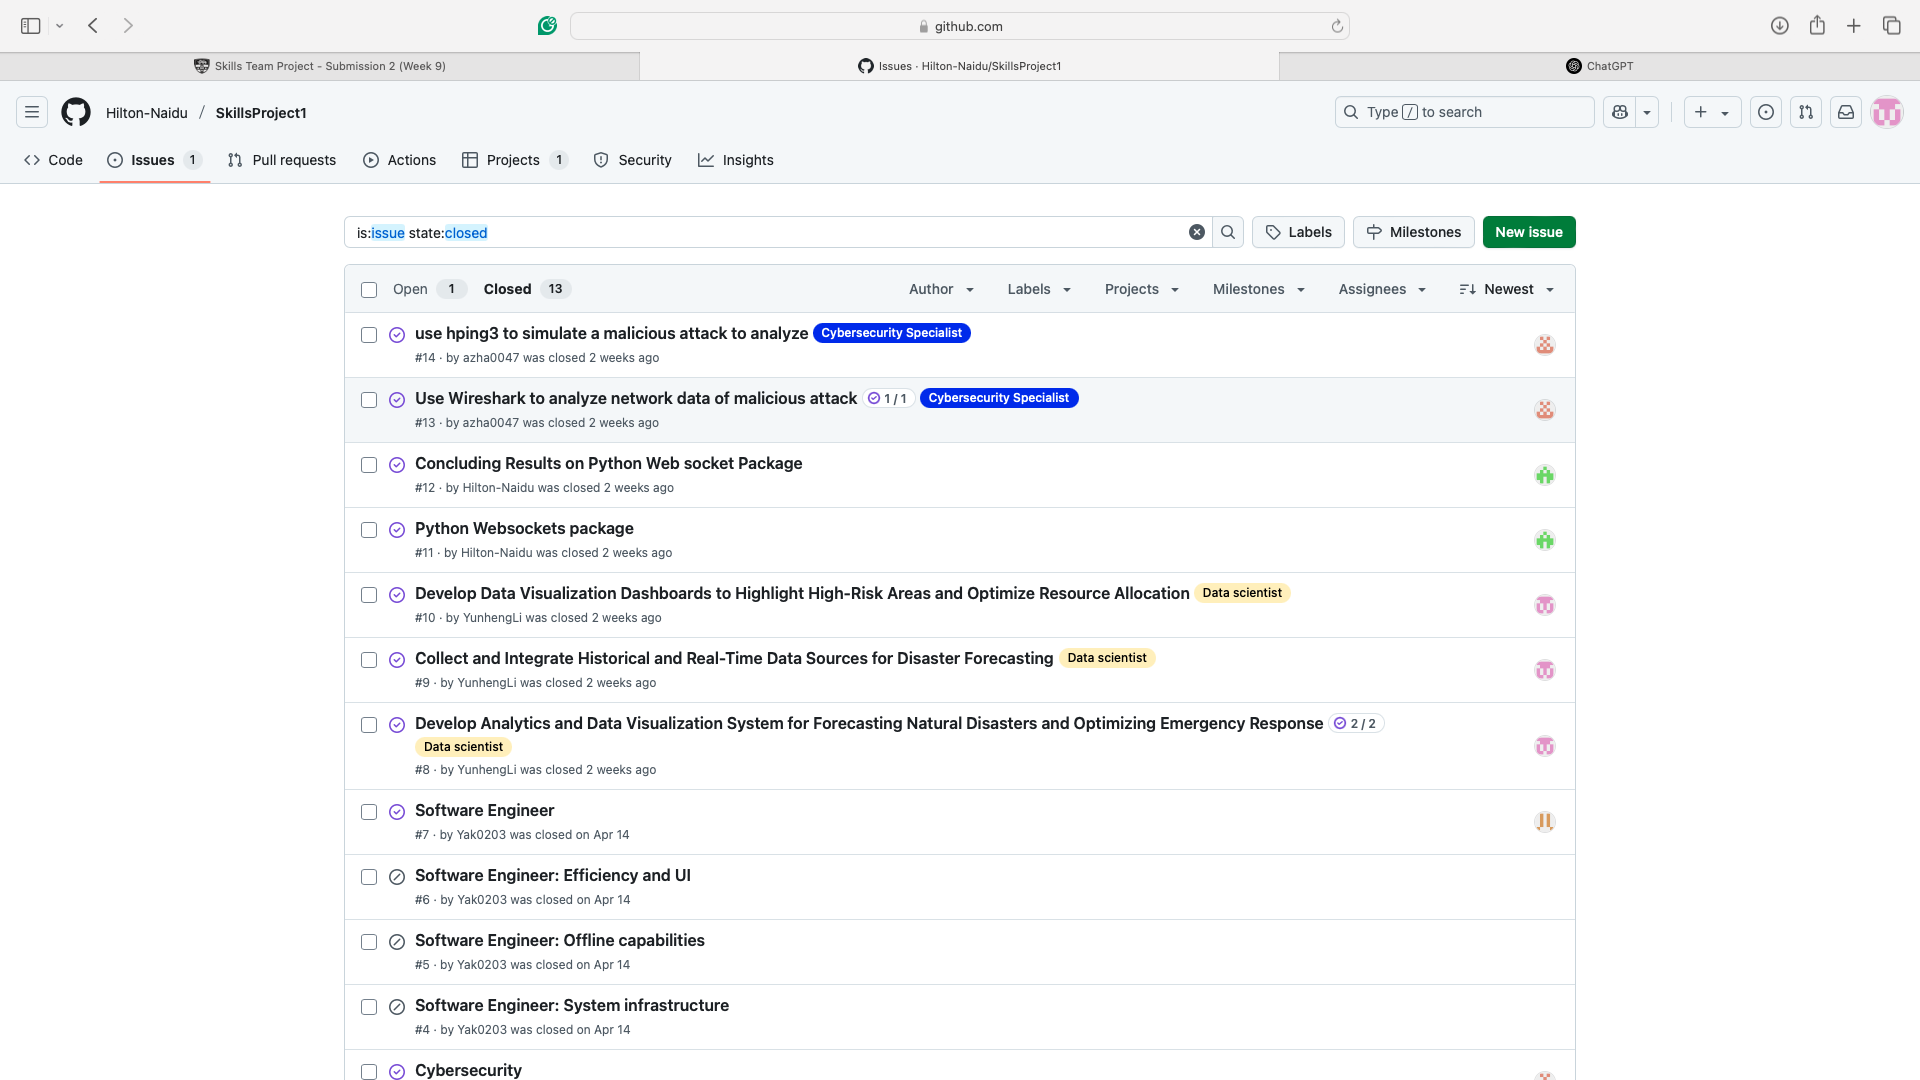
\includegraphics[width=10cm]{Field filter.png}
\caption{filtering for fields}
\end{minipage}
\begin{minipage}[t]{1.5\textwidth}
\centering
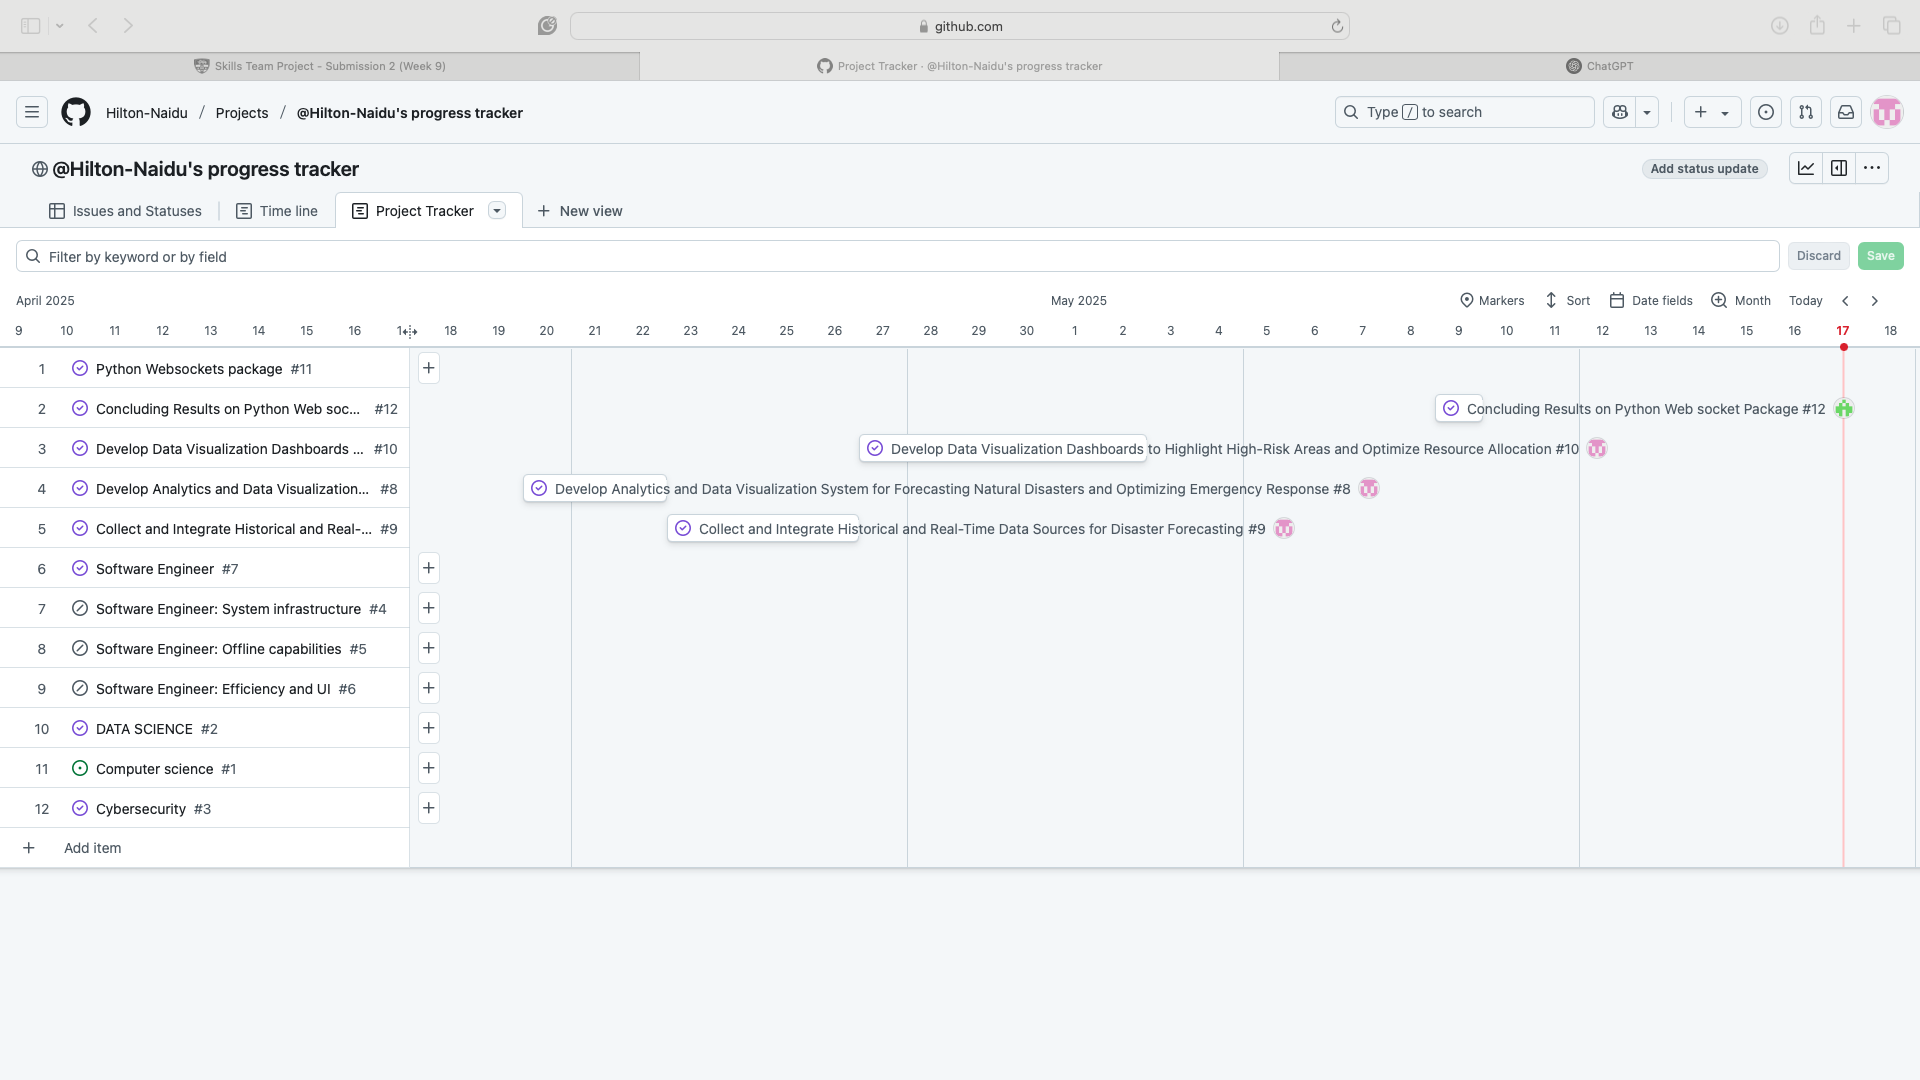
\includegraphics[width=10cm]{Tracker.png}
\caption{line chart}
\end{minipage}
\end{figure}


\subsection{Tools and Skills for \majA: \studA}

\subsubsection{Part A: Exploration of tech tools}

\textbf{NumPy} (Numerical Python) Python Websockets is a library (or package) which allow for performant and robust api communication for servers, based off the traditional HTTPS protocol of websockets which is widely used for its reliability and speed, some of it’s key features include:

\begin{enumerate}
    \item \textbf{Asynchronous WebSocket Server and Client Support}: Asynchronous programming is a incredibly powerful tool which allows for a system to act in response to events, rather than following a linear pattern. The package supports programming with the package asyncio which facilitates, allowing for non blocking communication, his is crucial for its scalability.
    \item \textbf{Full-Duplex Communication}: It enables simultaneous two way communication, allowing for a client to pull updates while simultaneously pushing new data to a server. This for example is highly useful for a live data system, such as an online game, where a client requires server updates, and other clients require server updates from different clients. Websockets maintain an open connection, unlike HTTP, which is request based.
    \item \textbf{Protocol Compliance and Error Handling}: The package also has compliance with RFC 6455 WebSocket protocol, which allows for the managing of handshakes, control frames, pings/pongs, and connection closing. It also has robust distributed systems, and mechanisms which ensure a graceful failure.
\end{enumerate}

This tool is important to the role of a Computer Scientist as it enables integration and development of real-time systems capable of sending and receiving online data. Python WebSocket supports real-time data feeds and low-latency communication, allowing experimentation with live user data. It also enables the design and testing of custom communication protocols over TCP. Async paradigms allow handling multiple clients from a central server and provide a lightweight mechanism to scale. This tool supports backend development for web applications using Python and async paradigms.

However, there are a few significant limitations or weaknesses of:

\begin{enumerate}
    \item \textbf{Single thread}: Python Websockets is a single threaded and Event-Loop Dependant. Since the library is designed around asyncio (single event loop) and does not support multithread processing, there is significant reduction in it’s capabilities to easily scale.
    \item \textbf{Lack of  features}: It lacks some significant high level features without extra work, such as broadcasting to multiple clients, session management, rooms, and automatic reconnection logic for clients. 
    \item \textbf{Security and privacy}: Security, while the package is capable of supporting secure websockets, it falls short in multiple other important areas, such as authentication layers (Jet, oAuth), Rate limiting, and message validation or encryption beyond TLS. 
\end{enumerate}


\subsubsection{Part B: Technical Skills and Analysis}

Your text goes here



% ========================================================

\subsection{Tools and Skills for \majB: \studB}

\subsubsection{Part A: Exploration of tech tools}

\section*{NumPy: Tool Description and Importance}

\textbf{NumPy} (Numerical Python) is a popular library in Python used for working with numbers and large sets of data \cite{harris2020}. Its main features include:

\begin{enumerate}
    \item \textbf{Multi-dimensional arrays}: NumPy makes it easy to create and work with arrays that have many rows and columns. It is much more effective than regular Python lists \cite{harris2020}.
    \item \textbf{Math operations}: It provides built-in ways to handling calculations like adding, multiplying, finding averages, or working with matrices effectively \cite{harris2020}.
    \item \textbf{Broadcasting and vectorization}: These features allow users to apply operations to the entire arrays at once, without writing complicated loops. By doing this, the code can become faster and cleaner \cite{harris2020}.
\end{enumerate}

NumPy is very important in fields like \textbf{Data Science (DS)}. In DS, it is the foundation for other tools like Pandas and SciPy, and helps with handling and analyzing big datasets. NumPy would help us quickly process large amounts of real-time and historical data, find high-risk areas, and help emergency teams plan better routes \cite{idris2013}.

However, even though NumPy is powerful, it has some limitations:

\begin{enumerate}
    \item \textbf{High memory use}: It can use a lot of memory when working with very large datasets, which may cause performance delays \cite{idris2015}.
    \item \textbf{No direct GPU support}: NumPy mainly runs on the CPU and cannot automatically use a GPU for faster calculations without other tools \cite{idris2015}.
    \item \textbf{Harder for beginners}: Some of the advanced features, like broadcasting, can be confusing if users are new to it \cite{idris2015}.
\end{enumerate}

In short, as a first-year data science student, I find NumPy to be an essential tool for building my skills in data analysis and problem-solving. Although I am still new to the field, using NumPy allows me to work with large datasets more easily and perform complex calculations than basic Python. In projects like forecasting natural disasters, NumPy provides me with a useful tool to handle real-world data effectively and accurately. Despite some difficulties mentioned above, like high memory use, which is challenging for beginners, I still believe that learning NumPy is an essential step toward becoming a strong data scientist who can contribute to solving complex problems.


\subsubsection{Part B: Technical Skills and Analysis}

\begin{figure}[htbp]
\centering
\begin{minipage}[t]{1.5\textwidth}
\centering
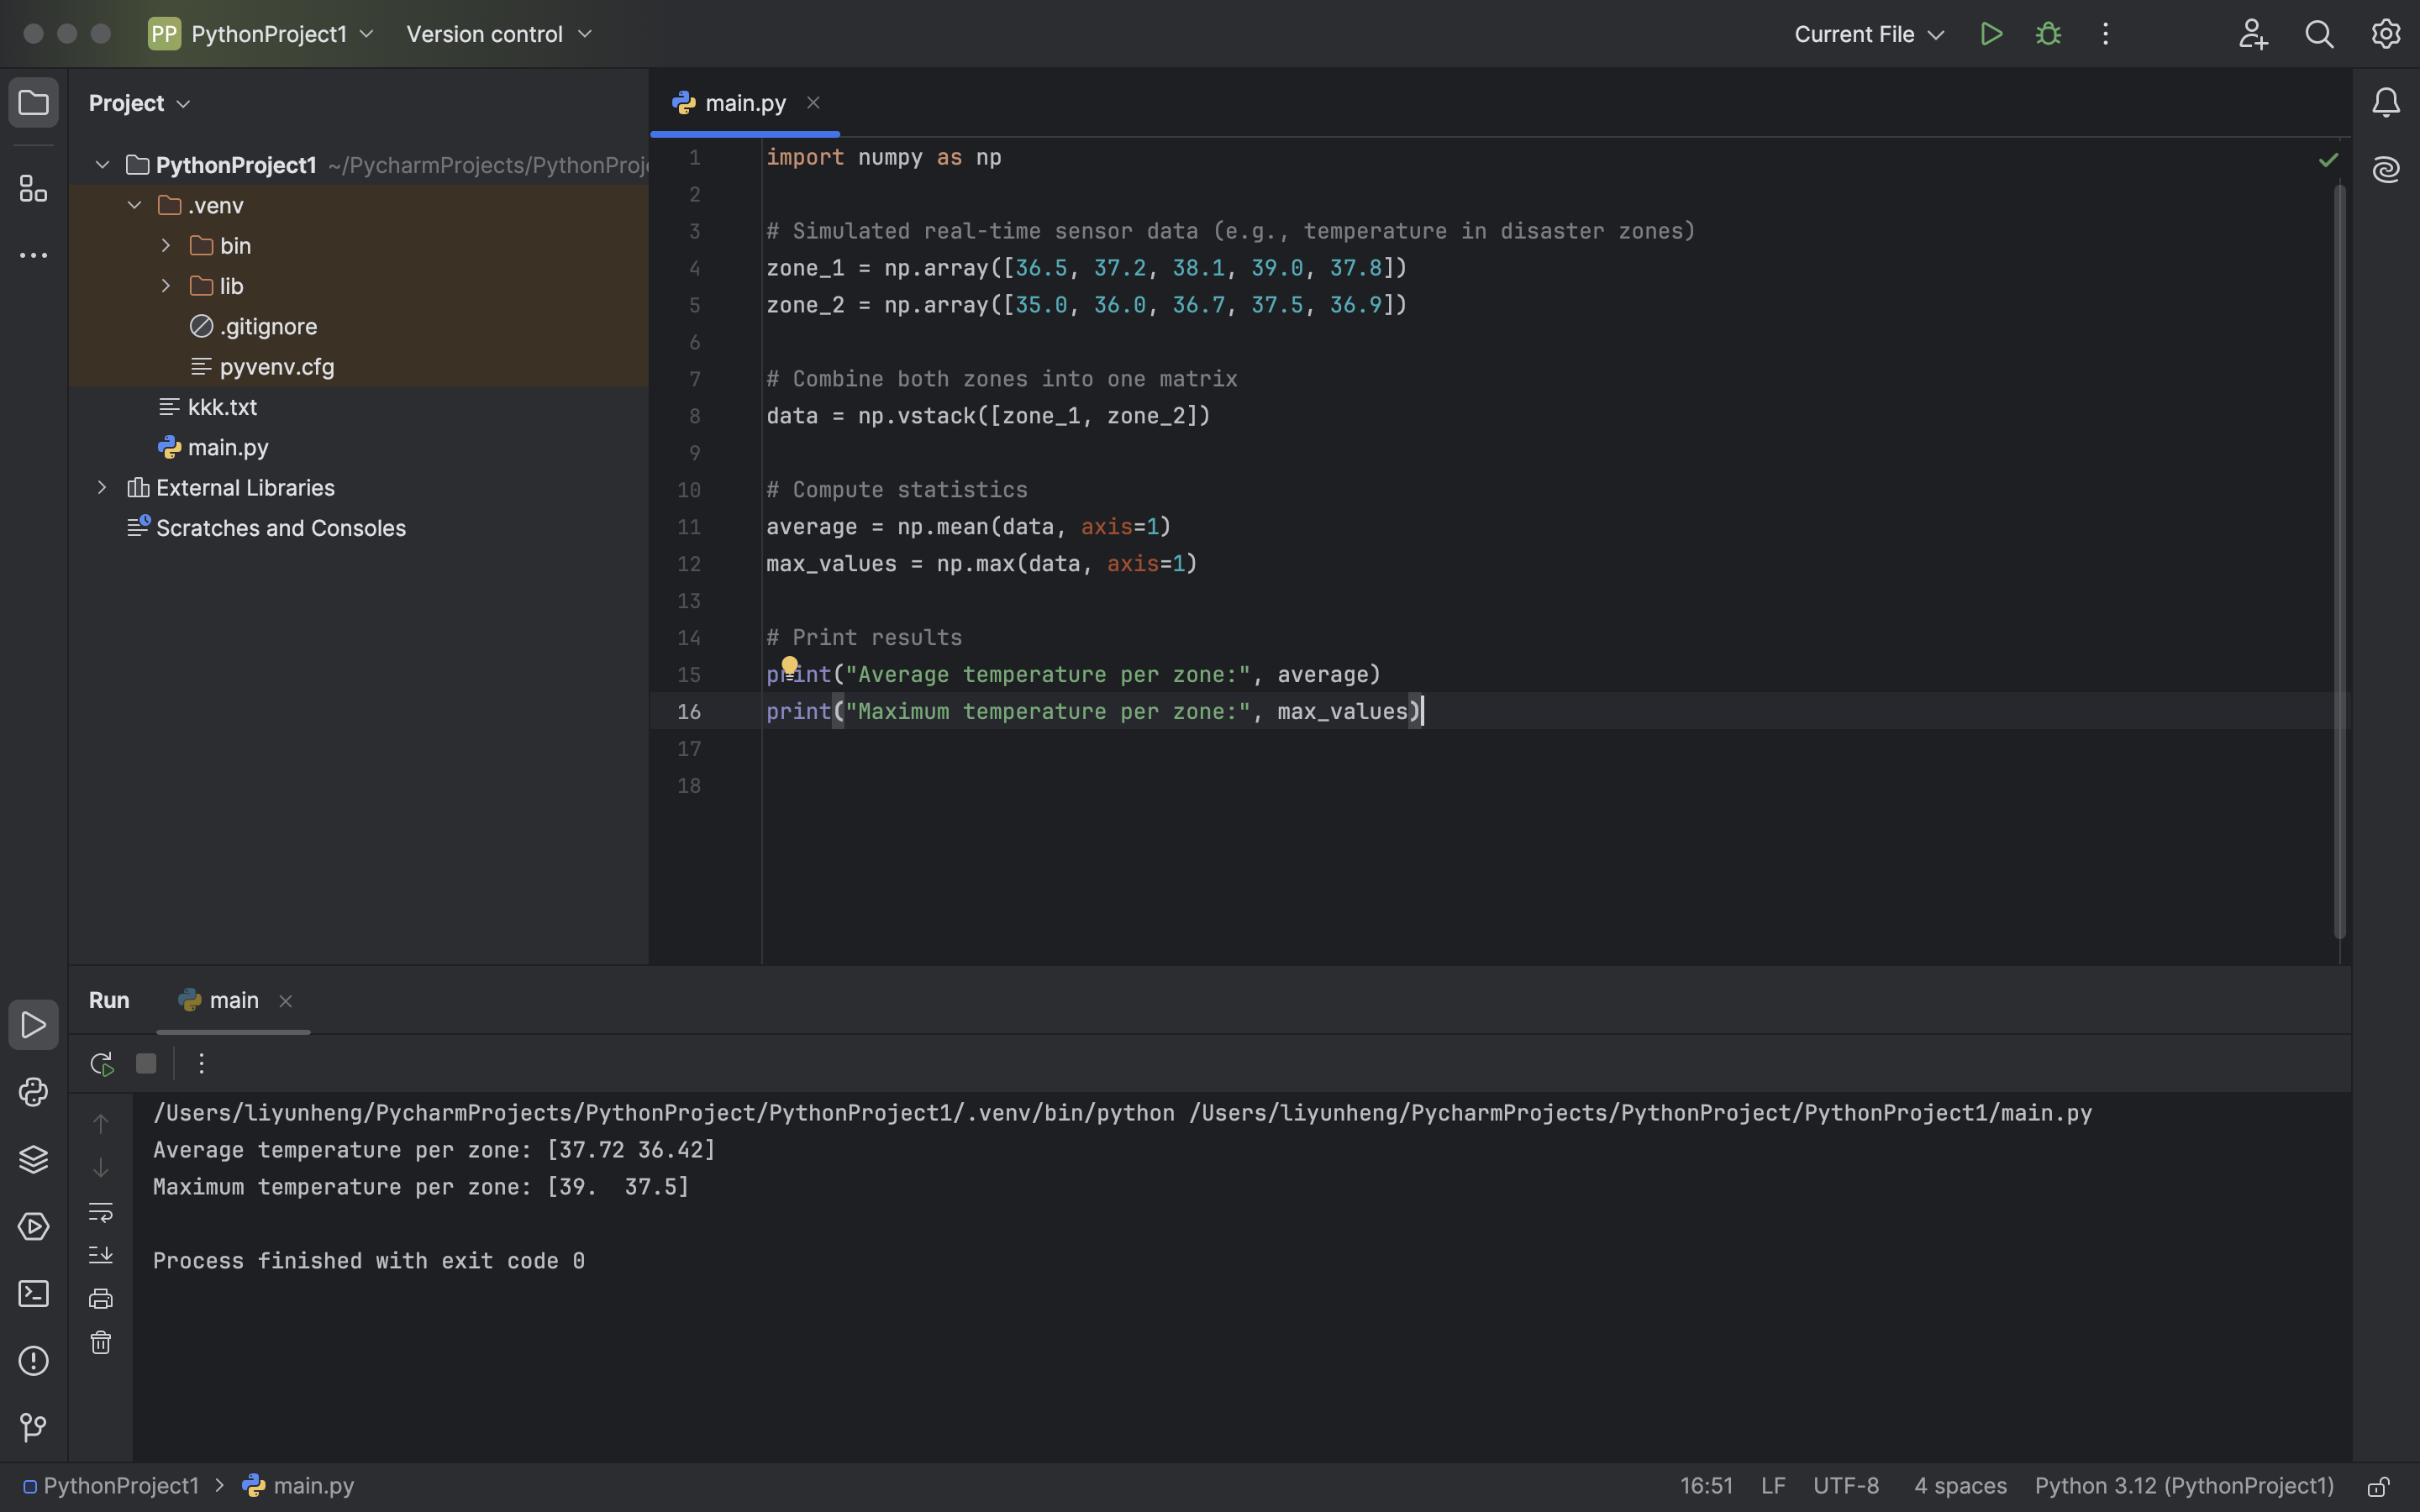
\includegraphics[width=10cm]{Numpy.png}
\caption{Numpy}
\end{minipage}
\end{figure}


Tool Implementation and Reflection

As part of the advanced component of our skills project, I explored NumPy, a Python-based library essential for numerical computing. I began by reviewing official documentation and experimenting with basic array manipulation. For the disaster response scenario, I simulated temperature readings from two affected zones and used NumPy to compute averages and peak temperatures. Initially, I struggled with understanding how multi-dimensional arrays worked in NumPy, especially using functions like vstack() and axis-based calculations. However, through practice and debugging, I overcame these challenges and became more confident with slicing, aggregating, and reshaping arrays.

One major insight I gained was how efficient NumPy is compared to regular Python loops — especially in time-critical applications like real-time disaster monitoring. This is highly relevant to my data science major, where large datasets must often be processed quickly and reliably. Learning NumPy has improved my ability to perform such tasks in a structured and optimized way.

In the context of disaster response, this tool becomes indispensable. Whether it's processing historical climate data, integrating live sensor streams, or modeling resource allocation, NumPy empowers responders to make timely, data-driven decisions. It can support early warning systems, hotspot detection, and even forecasting, making it a core part of any analytics pipeline in emergency situations. Ultimately, I realized that mastering such libraries is not only an academic requirement but a practical necessity for building intelligent, real-world solutions.


% ========================================================

\subsection{Tools and Skills for \majC: \studC}

\subsubsection{Part A: Exploration of tech tools}

Python Websockets is a library (or package) which allow for performant and robust api communication for servers, based off the traditional HTTPS protocol of websockets which is widely used for its reliability and speed. 


Asynchronous WebSocket Server and Client Support
Asynchronous programming is a incredibly powerful tool which allows for a system to act in response to events, rather than following a linear pattern. The package supports programming with the package asyncio which facilitates, allowing for non blocking communication, his is crucial for its scalability. 


Full-Duplex Communication
It enables simultaneous two way communication, allowing for a client to pull updates while simultaneously pushing new data to a server. This for example is highly useful for a live data system, such as an online game, where a client requires server updates, and other clients require server updates from different clients. Websockets maintain an open connection, unlike HTTP, which is request based. 


Protocol Compliance and Error Handling
The package also has compliance with RFC 6455 WebSocket protocol, which allows for the managing of handshakes, control frames, pings/pongs, and connection closing. It also has robust distributed systems, and mechanisms which ensure a graceful failure.


\subsubsection{Part B: Technical Skills and Analysis}

Your text goes here



% ========================================================

\subsection{Tools and Skills for \majD: \studD}

\subsubsection{Part A: Exploration of tech tools}

Wireshark is an open–source application used for analysing network traffic \cite{soepeno2023}. It enables the user to capture and inspect the packets from a network so they can troubleshoot and analyse the network in real time:

\begin{itemize}

	\item Wireshark provides tools to dissect packets for detailed network analysis, for diagnosing security threats and optimising network communications \cite{soepeno2023}.

	\item Real time network analysis using Wireshark can assist analysts in assessing trends and methodologies of attacks and create proactive response strategies and allow for faster detection of future attacks \cite{soepeno2023}.

	\item Wireshark provides extensive tools for capturing and logging network traffic with capture filters and display filters as well as logging traffic and specific intervals \cite{banerjee2010}. These features provide a lot of flexibility for users

\end{itemize}

Wireshark is widely used in the cybersecurity industry for the analysis of network security \cite{soepeno2023}. Specifically, it allows security analysts to perform detailed live analysis of network data at a packet level, allowing them to detect malicious activity, troubleshoot problems, and optimize network protocols \cite{banerjee2010}. Despite these upsides, there are some downsides to using wireshark:

\begin{itemize}

	\item While Wireshark can be used to detect suspicious activity on a network, it does not have the capability to automatically detect and create an alert when suspicious activity is detected \cite{mabsali2023}.

	\item Real time packet capture can be resource intensive to perform, particularly on busy networks with high traffic \cite{alizan2024}.

	\item Wireshark is limited to monitoring the traffic on networks that pass through the network interfaces of the machine that it is being used on, making remote monitoring more difficult \cite{alizan2024}.

\end{itemize}

In summary, Wireshark is a powerful network analysis tool that is a staple in the cybersecurity industry, and will be an important tool for me as I develop the skills to solve future cybersecurity challenges.

\subsubsection{Part B: Technical Skills and Analysis}

\begin{center}
	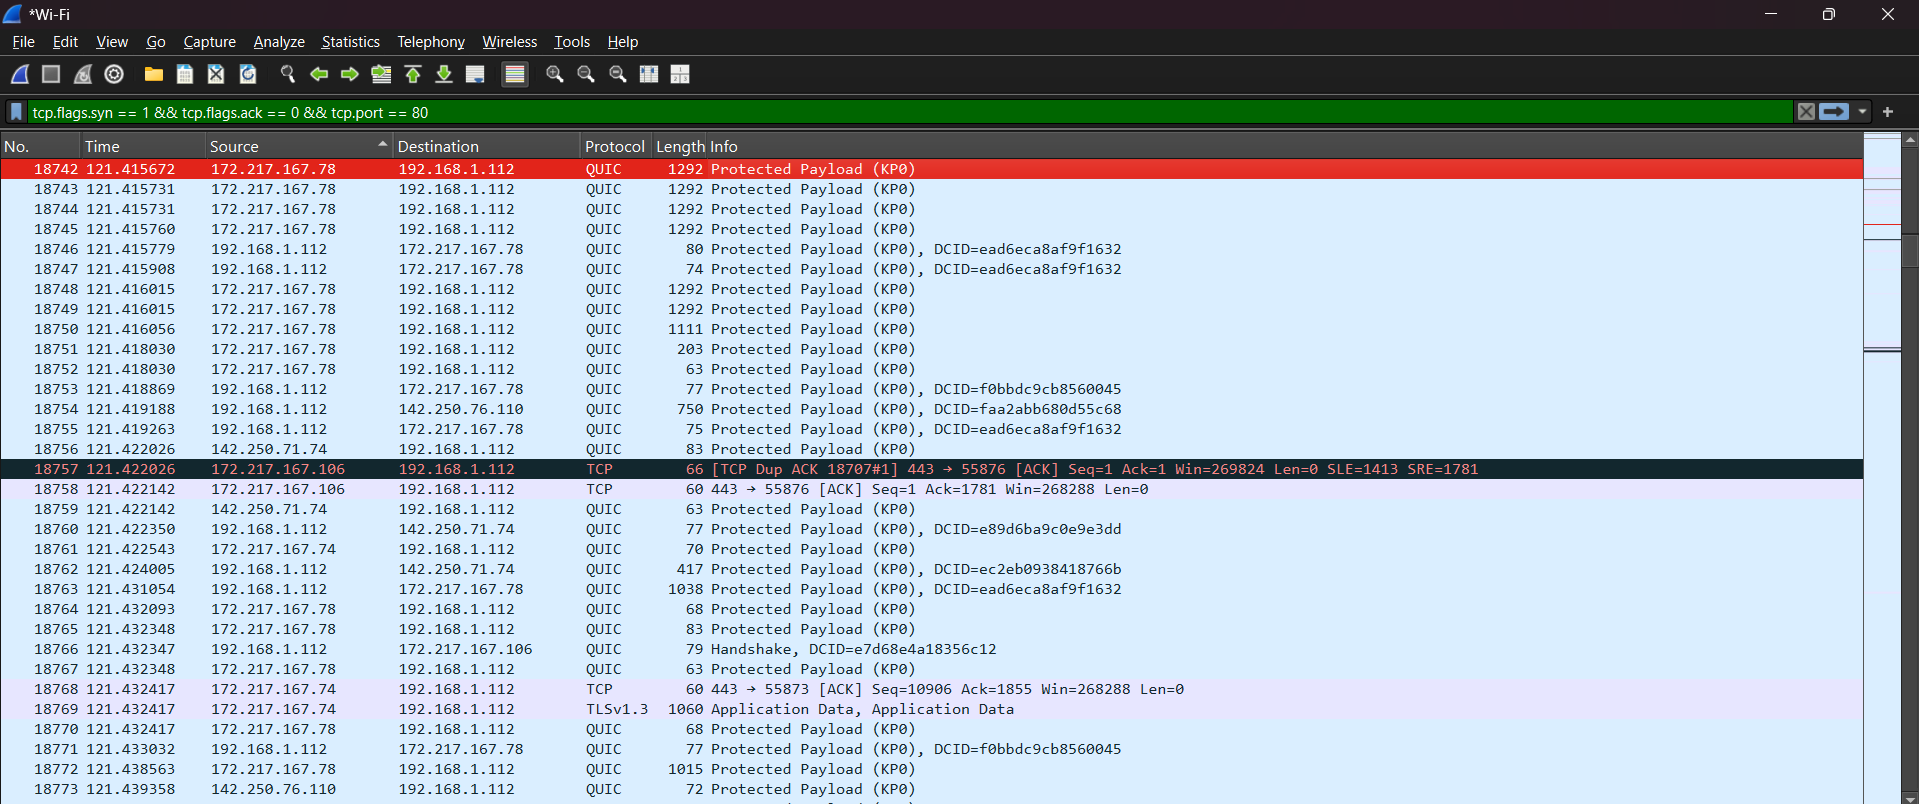
\includegraphics[width=0.5\textwidth]{wireshark1.png} \\
	normal network data \\

	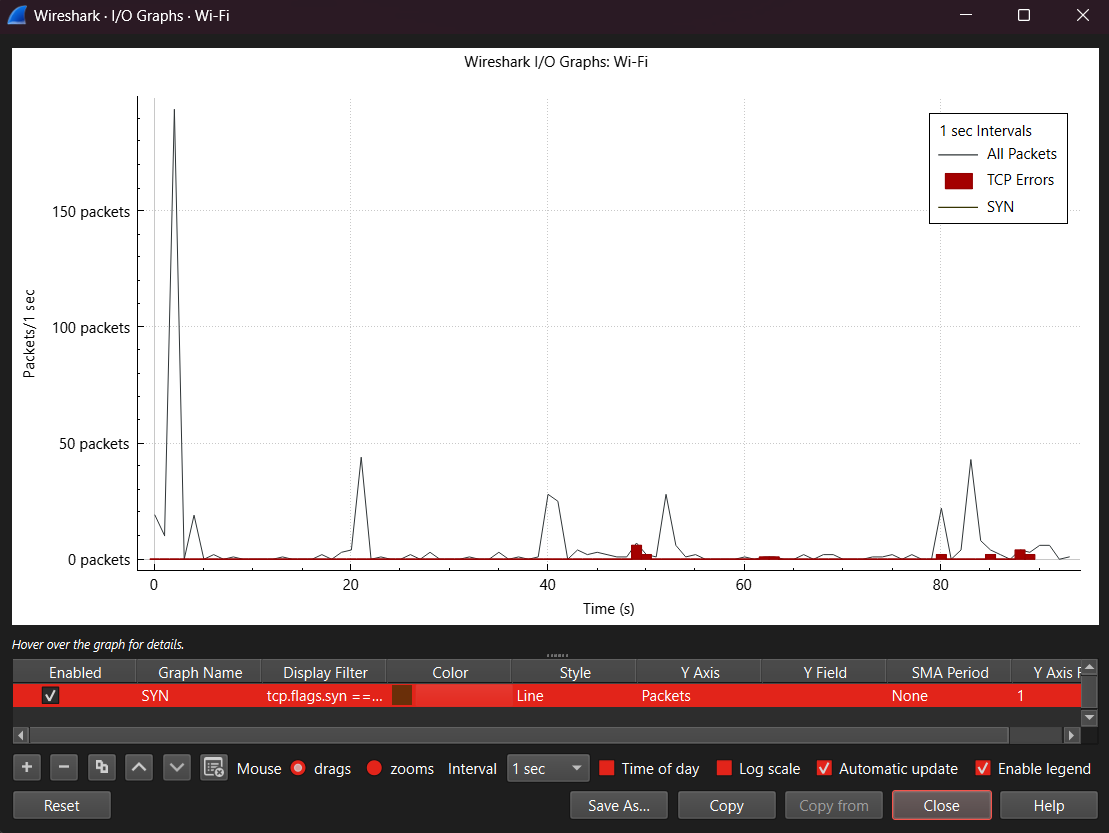
\includegraphics[width=0.5\textwidth]{wireshark2.png} \\
	normal network graph \\

\end{center}

As part of my investigation of Wireshark, I simulated the detection process of a malicious attack using Wireshark. To do this, I used hping3, a network tool that can be used to send custom TCP/IP packets, and I used this to simulate a DoS attack by sending a large amount of SYN packets to my test machine. I ran the command \texttt{sudo hping3 -S -p 80 –flood [ip]} to send a flood of SYN packets to my test machine. I filtered for the packets from the attack using \texttt{tcp.flags.syn == 1 \&\& tcp.flags.ack == 0} then I monitored the change in activity in Wireshark using an I/O graph.

\begin{center}
	
	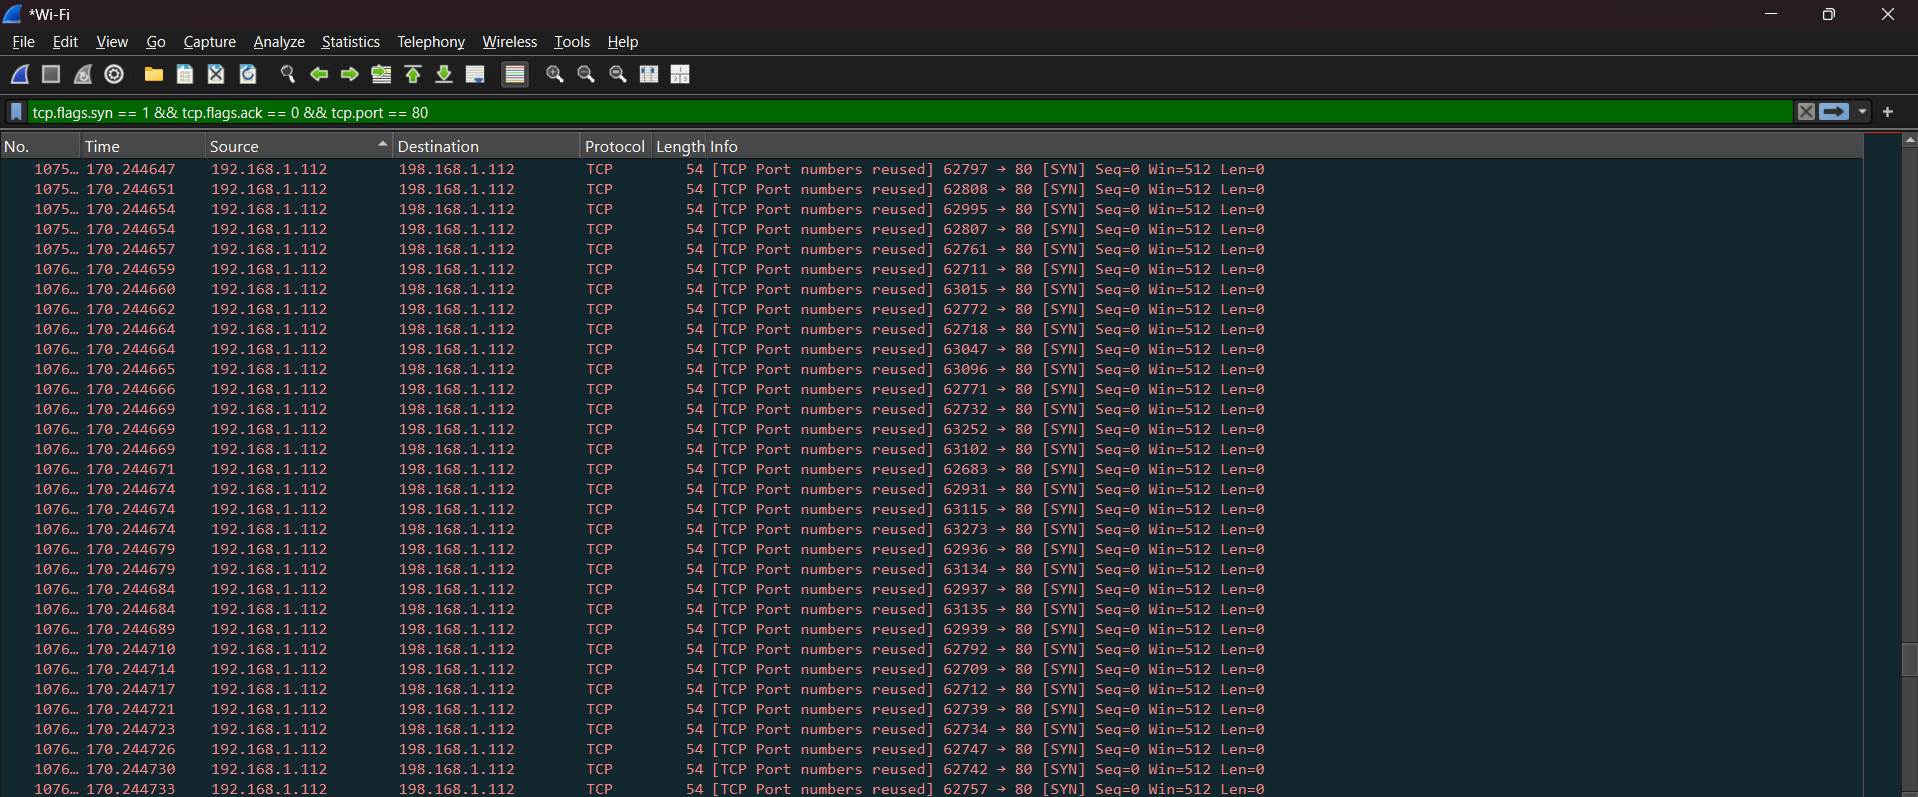
\includegraphics[width=0.5\textwidth]{wireshark3.png} \\
	SYN flood network data \\ 

	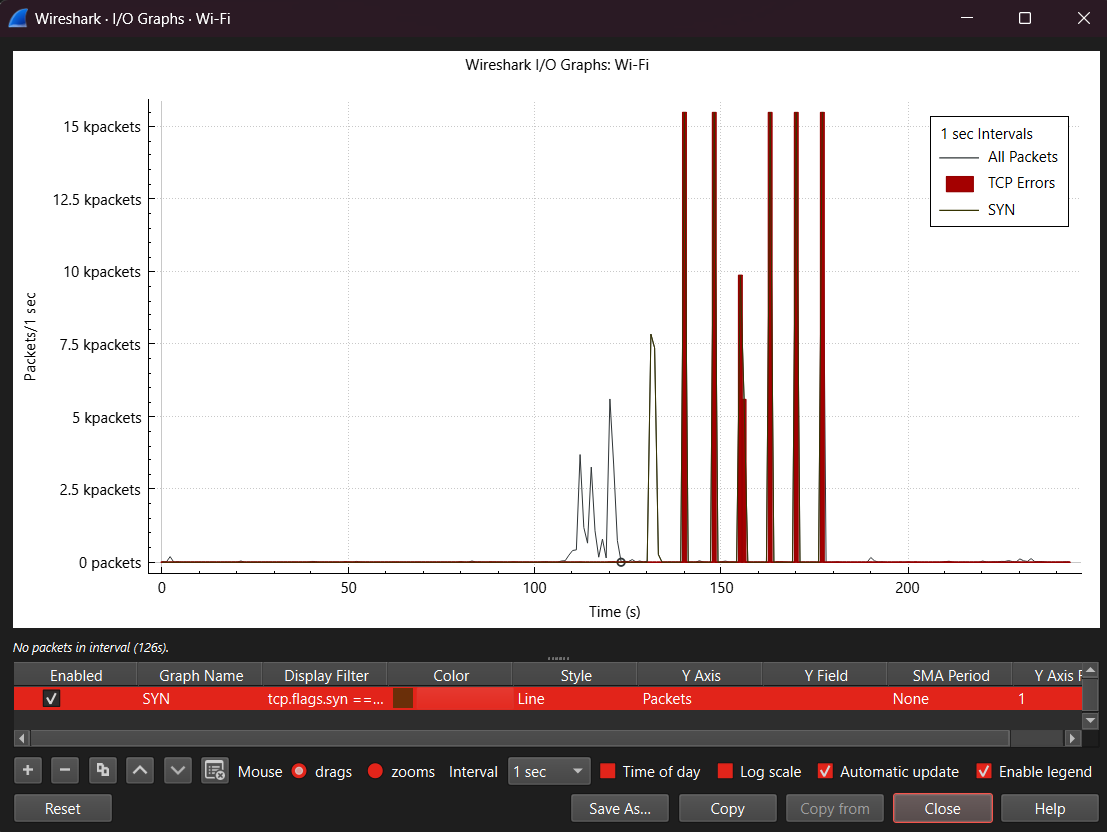
\includegraphics[width=0.5\textwidth]{wireshark4.png} \\
	SYN flood graph \\

\end{center}

In learning Wireshark, I first familiarised myself with basic network concepts such as packet structure and network protocols before learning the intricacies of Wireshark and how to use it. Initially, I found the interface overwhelming and struggled to isolate the relevant packets within the large volume of captured data. To overcome this, I relied heavily on online resources, including video tutorials, official documentation, and user forums. Through this process, I learned how to effectively use Wireshark to filter and interpret network traffic and represent it visually in graphs. This hands-on experience reinforced how essential tools like Wireshark are for diagnosing complex problems and maintaining secure systems in professional cybersecurity settings.

In a disaster response scenario, Wireshark could be used to monitor critical networks so that they can be proactively protected from any issues and malicious attacks that could happen. By identifying unusual patterns or unauthorized activity on the network, cybersecurity analysts could respond quickly to potential threats, ensuring that vital information reaches the right people without interruption. It could also be used during the development of a disaster response network as a tool to analyse and optimize network traffic so it can handle high traffic scenarios \cite{soepeno2023}. 

%=======================================================================================

\newpage
\section{Submission contribution overview}

For each submission, outline the approach taken to your teamwork, how you combined the various contributions, and whether there were any significant variations in the levels of involvement. (Target = $\sim$100-300 words).

\subsection{Submission 1 contribution overview}

For the completion of this submission, we all worked on our indervidual parts, and we all also attended the the group meeting where we collaberativly worked to come up with a plan and design our solution. The group response was written by Hilton Naidu. We all indervidually used Git and LaTex MikTex, we also all indervidually assigned ourselves tasks to complete. The final compilation and submission was done by Li Yunheng. This responses was written by Hilton Naidu. 

\subsection{Submission 2 contribution overview}

For Submission 2, we primarily worked independently due to the individual nature of the assigned tasks and the differing aims of team members. While we maintained communication to ensure overall alignment, each member was responsible for their own contribution. The Git chart was created by Hilton Naidu. The response was written by Li Yunheng, who also managed the final submission process.

\subsection{Submission 3 contribution overview}

As above, for submission 3


%=======================================================================================

\newpage

\bibliographystyle{IEEEtran}
\bibliography{main}

\end{document}
\end{report}
